\chapter{Evaluation}
\label{cpt:evaluation}
\todo{Bringe in richtige reihenfolge}
In this chapter, the developed system is evaluated with respect to various criteria.
At first, an overview about the utilized \abr{DDS} subset is described and the necessity of each feature is justified.

This is followed by an system evaluation where both the system's hardware structure as well as the implemented software are evaluated.
Within the implementation evaluation, all characteristics that correspond with the manner of how the software is implemented, are considered.
First, general system properties are analyzed, such as the time needed to send and receive messages or the maximum time the system can be without a leader.
This allows to answer fundamental questions about the system's reliability because the average time to synchronize the components can be derived.
Afterwards, metrics related to the execution of specific scenarios are examined.
These include the utilization of system resources on the one hand and the number of messages sent and received on the other.
From these metrics it can be seen at which points in time an increase in system performance can be expected and that enough resources are always available in the applied system.

\section{System Evaluation}
At first in this section, general system metrics are analyzed.
Afterwards, the system is analyzed while running and processing input messages from simulated scenarios.
For this purpose, three scenarios are simulated and processed one after the other and system characteristics such as resource utilization and exchanged messages are collected.

\subsection{General System Characteristics}
General system properties include those that are independent from input messages and the system's global state.
Such a general system property is the time that it takes to elect a new leader, from which the average time that the system is without a leader can be derived.
The election time is limited by the replica's computational resources and by the speed of data transmission.
The latter is also investigated in the following by measuring the time it takes to publish and read messages of different sizes through \abr{DDS} topics.
Finally, the resource utilization of the system in idle mode is examined.
In idle mode, the train is at a standstill and no input messages are evaluated.

\paragraph{Leader Election Time}
\todo{Redo measurements}
\begin{figure}[!hb]
	\centering
	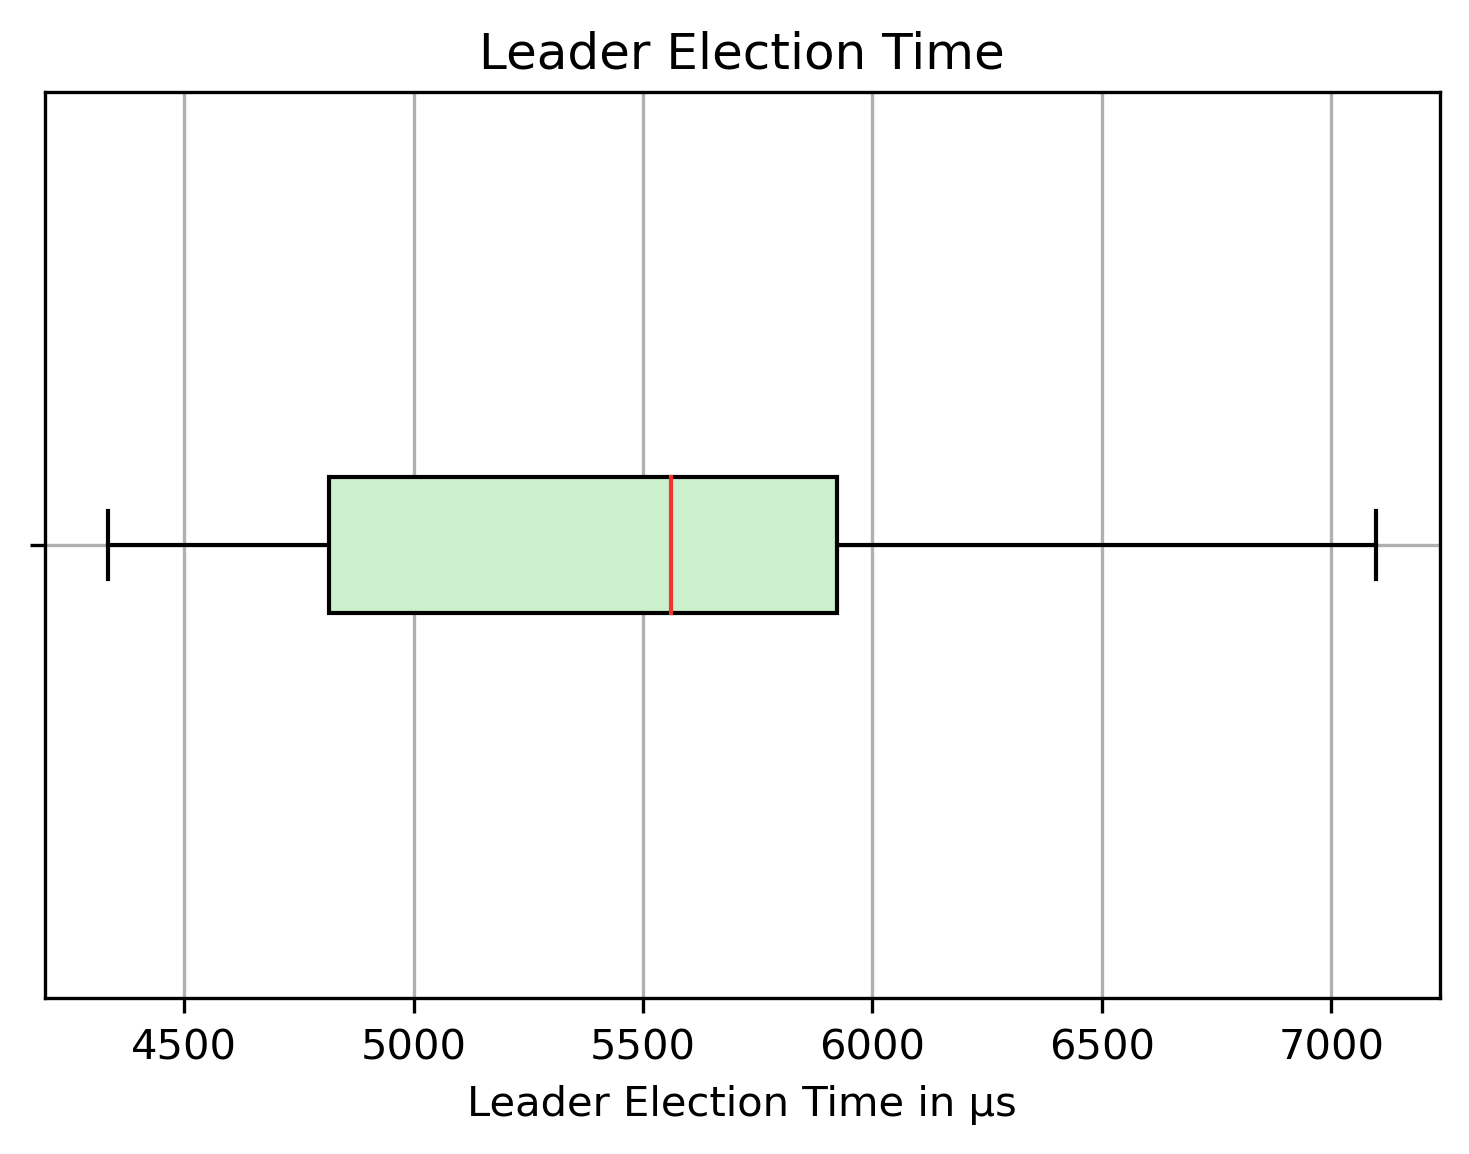
\includegraphics[width=0.75\linewidth]{images/plots/timeWithoutLeader}
	\caption{Time that the system is without a leader in each term for 20 terms. The average of 5472µs is marked by the red line.}
	\label{fig:PlotTimeWithoutLeader}
\end{figure}

When the system's leader crashes, the current \texttt{Raft} term ends and a new leader gets elected.
The leader election process consists of requesting and collecting votes from all replicas in the system.
In order to investigate how long the leader election process takes, the time for 20 elections was measured.
This has been done by starting a timer when a missing leader got noticed until a heartbeat message from a new leader was received.
The results can be seen in~\autoref{fig:PlotTimeWithoutLeader} and show that the process takes around 5500µs on average and at worst 7000µs.
However, since the system utilizes a timeout to detect an absent leader, the total time that the system is without a leader arises from the sum of the applied election timeout and the election duration from~\autoref{fig:PlotTimeWithoutLeader}.

\paragraph{Data Transmission Time}
\begin{figure}[!hb]
	\centering
	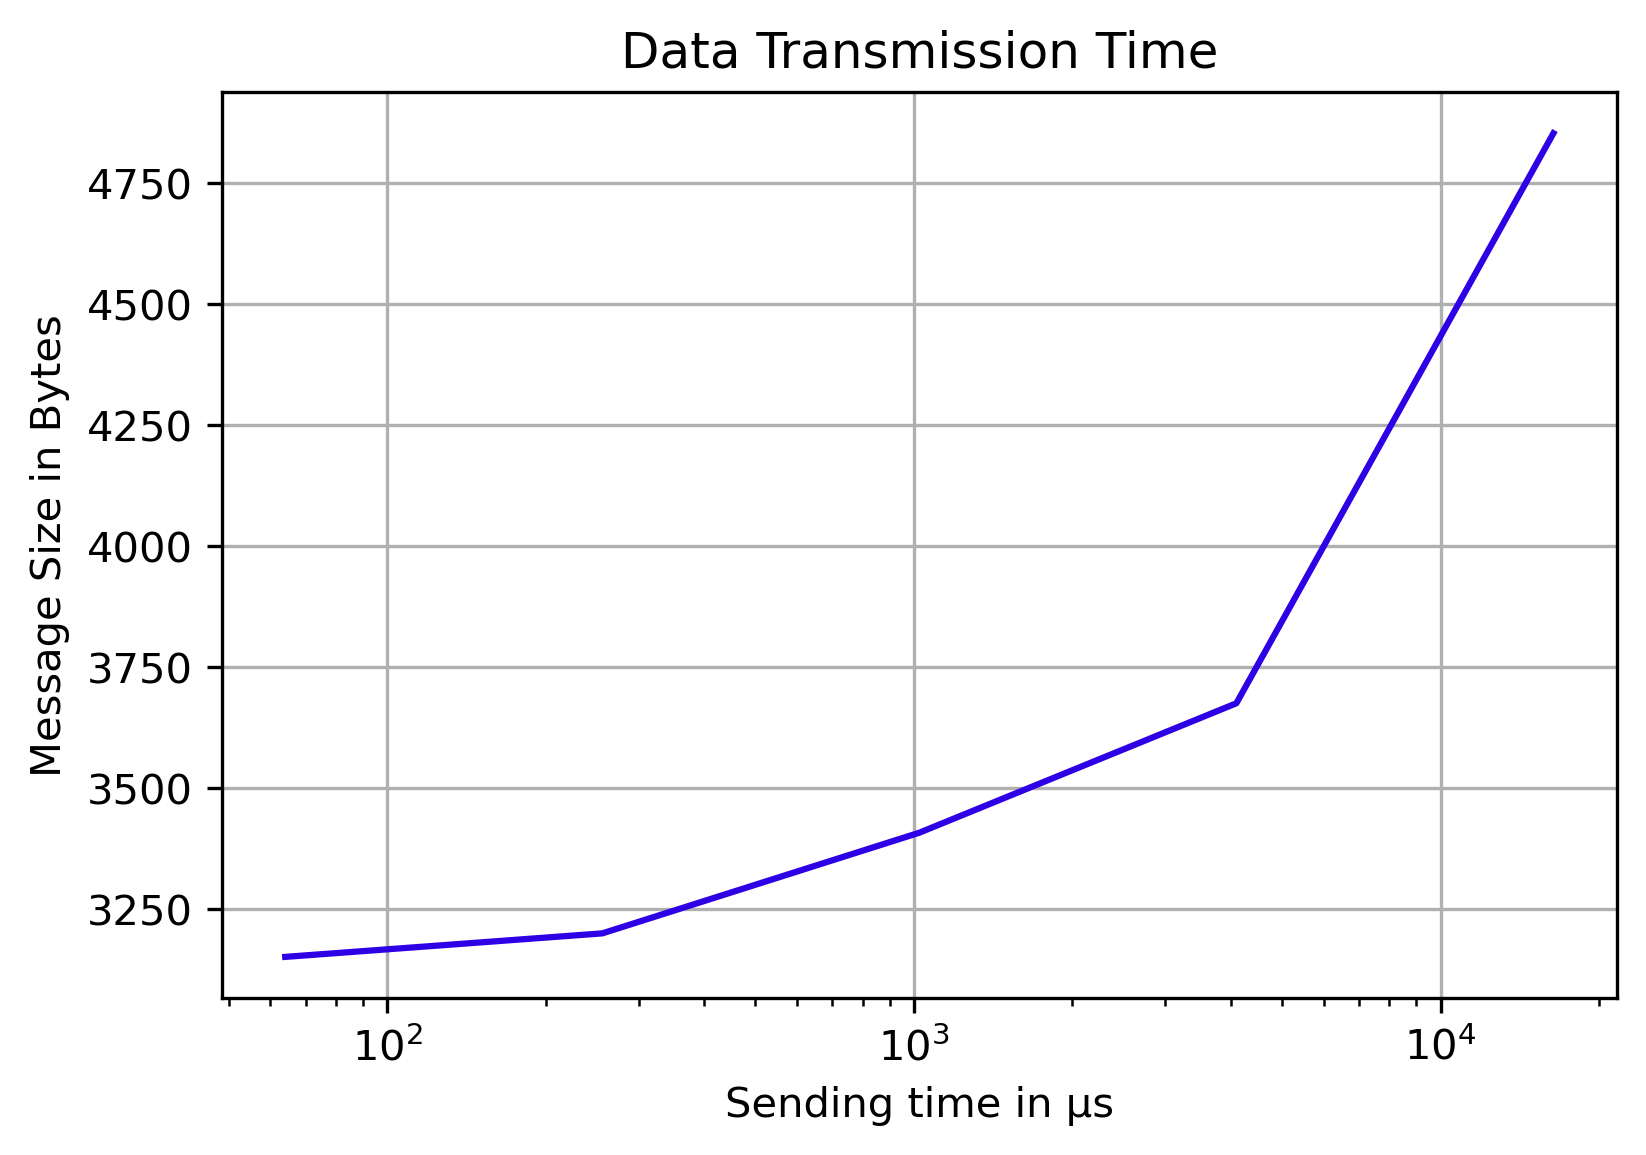
\includegraphics[width=0.75\linewidth]{images/plots/sendingTimes}
	\caption{Time that is required to transmit messages with different payload sizes via a \abr{DDS} topic. The times were determined by calculating the mean sending time out of 200 messages per payload size.}
	\label{fig:PlotSendingTimes}
\end{figure}

\begin{figure}[!hb]
	\centering
	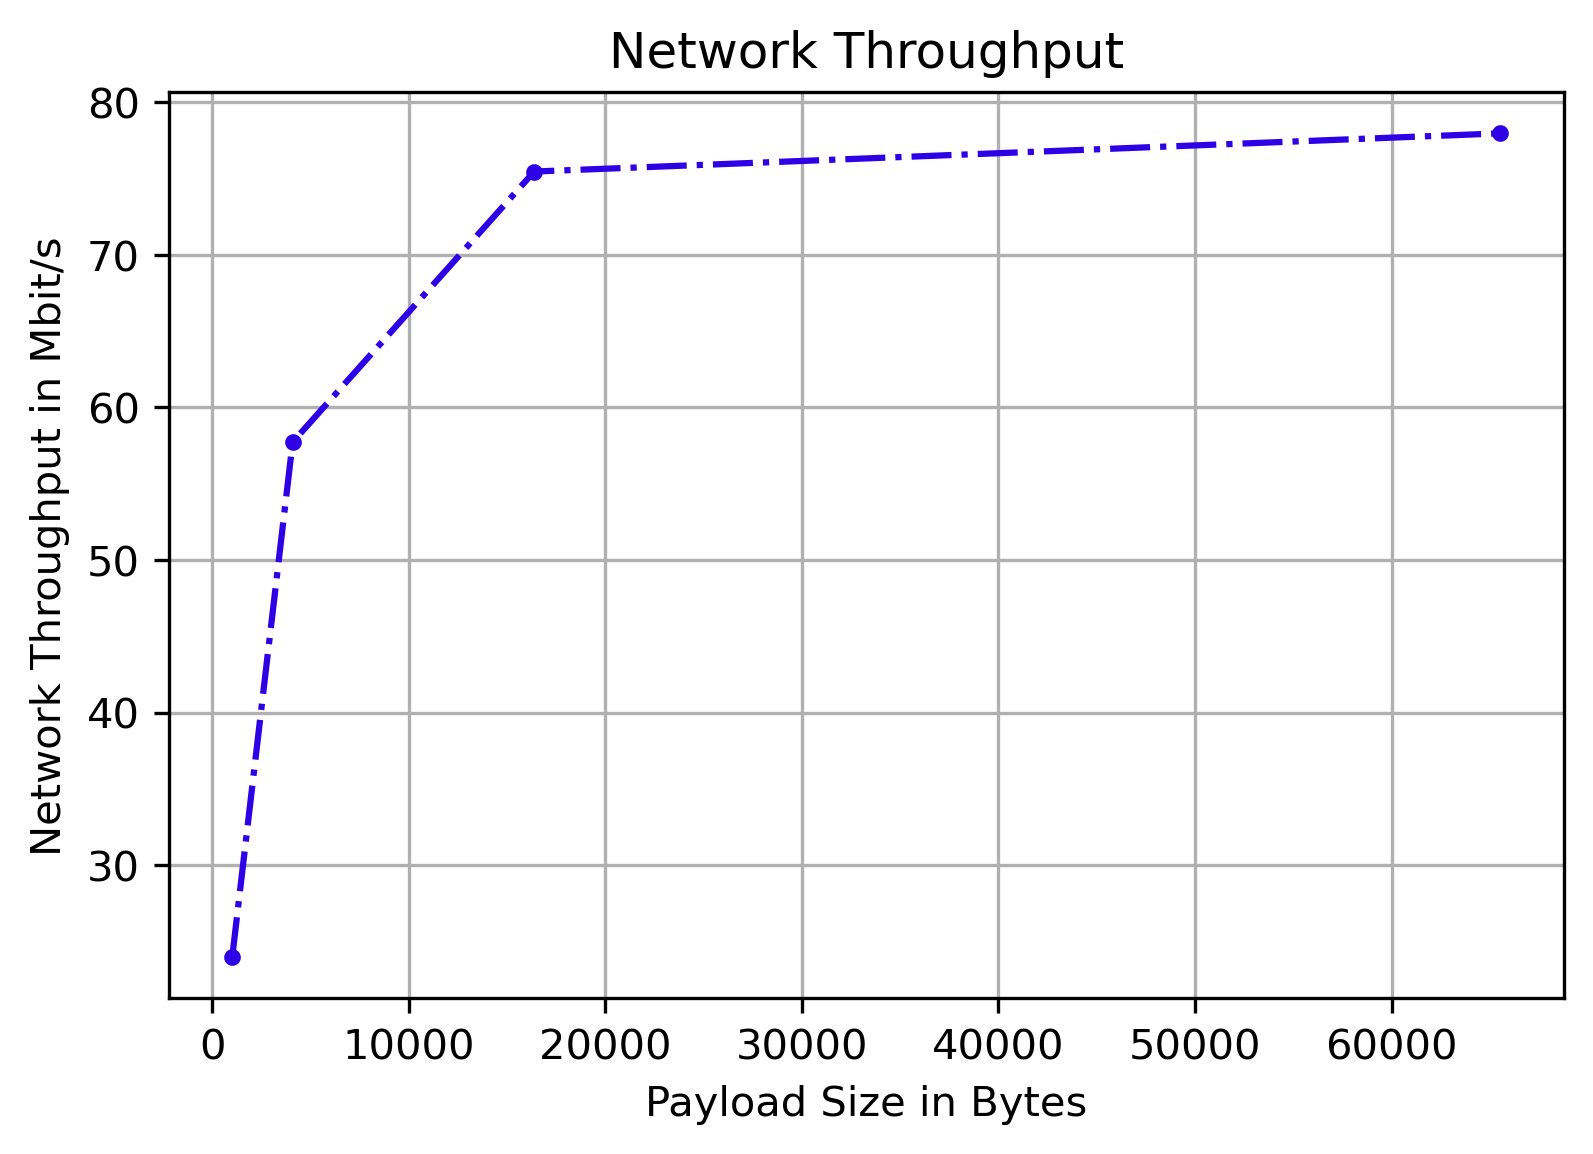
\includegraphics[width=0.75\linewidth]{images/plots/dataThroughput}
	\caption{Maximum supported data throughput. The throughput was measured with a program by ADLINK. On average, 56.5 Mbit/s is reached.}
	\label{fig:PlotDataThroughput}
\end{figure}

A end-to-end probing approach has been chosen to measure data transmission times, although a \abr{IP} \abr{TTL} technique has been proposed by~\cite{SinhaMeasureNetworkLatency}.
This is because the applied network has the same diameter for each node.
When a component publishes data to a \abr{DDS} topic, the middleware ensures that the data is transmitted to all registered subscribers.
In the system that is deployed for this thesis, data is transmitted via an \textit{Ethernet} connection.
The replicas are interconnected via a network switch that allows up to 2000 Mbit per seconds for each port.
On average, a data throughput of 56.5 Mbit/s is reached in the system, as depicted in~\autoref{fig:PlotDataThroughput}.
The data throughput has been measured with a dedicated program by ADLINK.

Further, the time that is required to publish and process a message with a certain payload size between two replicas via a \abr{DDS} topic is measured.
For bypassing clock skews in the system, a request/response approach is used, where one replica publishes a message with a certain payload size and waits until another replica confirms the message's receipt.
The receiving replica constantly checks for new messages and, as soon as it receives one, publishes a confirmation messages on another topic.
Any time that is required to send the confirmation message is negligible because it only consists of a 8-bit identification number that assigns it to a payload carrying message.
The results, which are shown in~\autoref{fig:PlotSendingTimes}, were determined by measuring the time that elapsed between sending a message and receiving the corresponding confirmation.
This process was repeated 200 times for each payload size and a mean was calculated.
What emerged is, that the transmission time is directly dependent on the published message's size.
\\

\begin{table}[h!]
	\begin{center}
		\caption{All topics that are utilized in the system have a certain data schema. From the resulting message size, the transmission time in the system can be calculated. The size and transmission time of the \texttt{AppendEntries} and \texttt{Input} depends on the length of the data sequence (\textbf{l}).}
		\label{tab:topicSendingTimes}
		\begin{tabularx}{\textwidth}{|X|X|X|}
			\hline
			\textbf{Topic} & \textbf{Message Size in Bytes} & \textbf{Expected Transmission Time in µs} \\
			\hline \hline
			AppendEntries & $12 + 4 * l$ & $0.402768 * l + 3219.11$ \\
			\hline
			AppendEntriesReply & 18 & 3219.7 \\
			\hline
			RequestVote & 8 & 3218.7 \\
			\hline
			RequestVoteReply & 13 & 3219.21 \\
			\hline
			Input & $4 + 4 * l$ & $0.402768 * l + 3218.3$ \\
			\hline
			ActivateSpare & 5 & 3218.40 \\
			\hline
			LinkedBalises & 6 & 3218.5 \\
			\hline
			TrainState & 41 & 3222 \\
			\hline
			MovementAuthority & 8 & 3218.7 \\
			\hline
		\end{tabularx}
	\end{center}
\end{table}

Each topic that is used in the system has a certain data structure, that is determined by its \abr{IDL} representation.
Using the data structure and the transmission times from~\autoref{fig:PlotSendingTimes}, the expected trasmission time for each topic can be calculated.
These expected transmission times are listed in~\autoref{tab:topicSendingTimes}.
The message sizes are based on the \textit{Revolution Pi}'s architectural characteristics.
In ADLINK's \texttt{OpenSplice DDS}, the \textit{short} \abr{IDL} datatype resolves to a \textit{short int} C type, \textit{long} resolves to \textit{int} for the C programming language, \textit{unsigned long long} resolves to \textit{unsigned long long int}, and the \textit{boolean} datatype resolves to an \textit{unsigned char}.
A \textit{double} \abr{IDL} datatype resolves to a \textit{double} C type.
The replica system's size characteristics for an \textit{short int} are two bytes, for an \textit{int} are four bytes, for an \textit{unsigned long long int} are eight bytes, for a \textit{double} are eight bytes, and for an \textit{unsigned char} is one byte.
The transmission time was calculated via the equation $transmissionTime(size) = 0.1100692 * size + 3217.9$ that has been derived by regression from the results in~\autoref{fig:PlotSendingTimes}.
For the \texttt{AppendEntries} and \texttt{Input} topic, the actual data size and thereby the expected transmission time depend on the data sequence's length. 

\todo{Was bedeutet das für das konkrete System}

\paragraph{Idle Resource Utilization}
\begin{figure}[!hb]
	\centering
	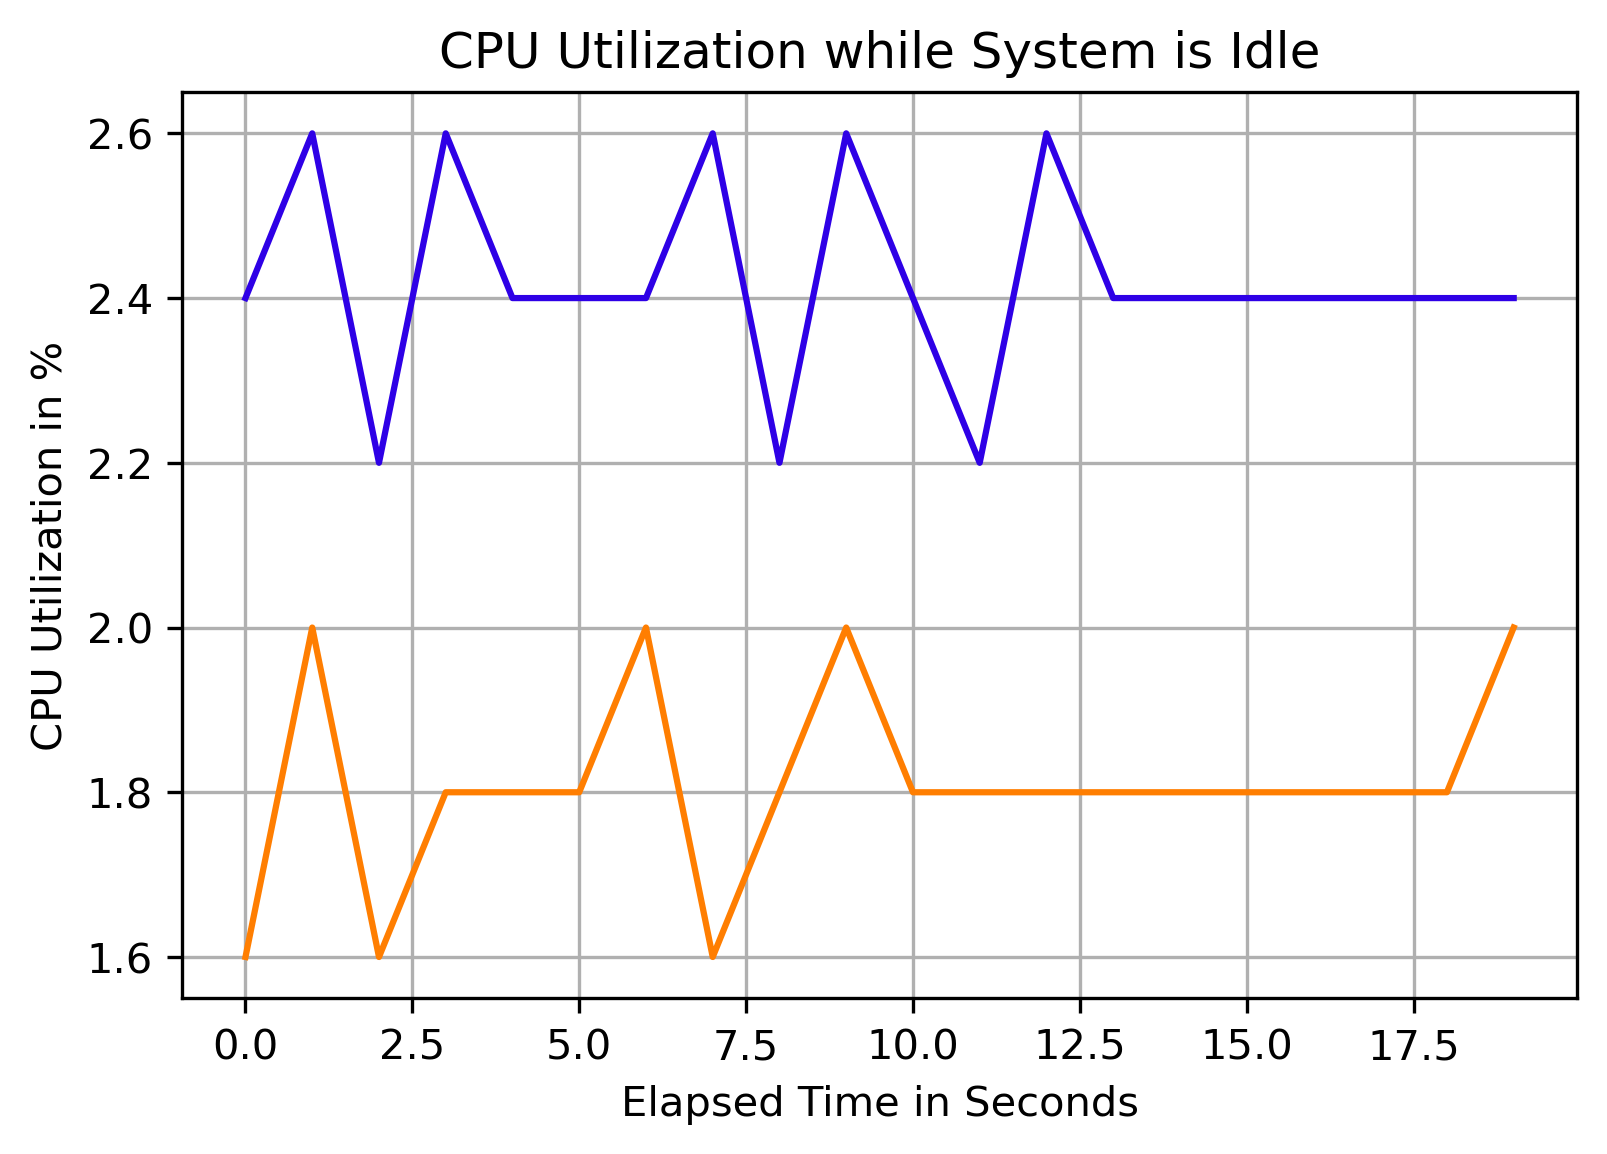
\includegraphics[width=0.75\linewidth]{images/plots/CPUUsageIdleTime}
	\caption{This plot shows the \glsentryfull{CPU} utilization in \% for both leader and follower in idle mode where only heartbeat messages are exchanged.}
	\label{fig:PlotCPUUsageIdleTime}
\end{figure}

In this paragraph, the utilized \abr{CPU} resources for both leaders and followers in idle mode are examined.
Measurements were made with \textit{pidstat}, a tool that monitors individual tasks that are managed by the \abr{OS} kernel.
\\

In idle mode, the train is not driving and only heartbeat messages are exchanged between the leader and its followers.
The \abr{CPU} usage for both a leader and a follower in idle mode are depicted in~\autoref{fig:PlotCPUUsageIdleTime}.
It can be seen that the leader's hardware utilization is consistently higher than the follower's.
On average, the follower utilized 1.81\% in 90 seconds, while the leader utilized 2.42\% of the applied \abr{CPU}.
In system mode, 0.21\% are used for the leader and 0.25\% for a follower on average.
For user mode, the leader utilizes on average 1.0\%, while a follower uses 0.66\%.
This can be explained by the fact that the leader has more responsibilities in idle mode.
It not only periodically sends heartbeat messages, but also observes whether the train has a valid \abr{MA} and can start driving.


\subsection{System Characteristics in Operative Mode}

\begin{table}[h!]
	\begin{center}
		\caption{A Python program is used for automatic integration testing. The scenarios that are traversed in the process differ in the relation of linked and unlinked balises and their expected outcome.}
		\label{tab:simulatedScenarios}
		\begin{tabularx}{\textwidth}{|X|X|X|}
			\hline
			\textbf{Name} & \textbf{Number of balises/linked balises} & \textbf{Expected behaviour}\\
			\hline \hline
			Reach End of \abr{MA} & Three/Three & All balise telegrams are evaluated correctly and the train stops at the \abr{MA}'s end. \\
			\hline
			Unlinked Balise & Three/Two & The train stops when the third and unlinked balise is encountered. \\
			\hline
			Balise not where expected & Three/Three & The actual position of the last balise does not correspond with its linked position. The train stops when this balise is encountered. \\
			\hline
		\end{tabularx}
	\end{center}
\end{table}

In the following, the system's characteristics are measured and evaluated while it is in operative mode.
Operative mode means, that the train's movement is supervised, input messages are evaluated, and a voting is performed based on all replica's decisions.
In order to evaluate the system in operative mode, three scenarios are simulated using the simulator which has been described in~\autoref{subsec:ScenarioSimulation}

All three scenarios include a \abr{MA} of equal length and three balises.
However, they differ in the number of linked balises and the balise's positions.
An overview about the simulated scenarios and the system's expected behaviour is given in~\autoref{tab:simulatedScenarios}.
\\

In a second experiment, the system's hardware resource utilization is recorded.
This data set provides information on whether the used hardware components can withstand the demands of the implemented system.
\\

Because the trips are simulated, a reproducible test environment is created.
This has the benefit that it allows the system to be automatically tested and facilitates the measurement of characteristics under equal circumstances.
Further, data reproducibility allows to make changes to the system and evaluate how it performs compared to other versions.
The simulation allows to test the system in different situations without using and jeopardising real trains and trackside components.
An automatic test and evaluation process allows to validate the system under varying circumstances and to replicate tests.
Thus, the system's correctness and reliability can be shown because repeated tests enhance the chance to find synchronization mistakes.
Although it is difficult to to approve the system's \abr{SIL}, its behavioural reproducibility can be shown.

In order to facilitate automatic integration testing, the on-board unit's system logic has been patched to write the system's decisions to input messages and braking curve ovservations into an evaluation file.
For each decision, the train's current position, the decision whether the train should brake or continue driving, the last encountered balise, and a reason are exposed.
Finally, a script assesses all evaluation files and compares the system's reactions to the desired behaviour.
\\

For every message that is published or received by a replica, an entry is written into another file.
Thereby, not only the system's final decision, but also the replica's synchronization to come to an agreement can be understood.

However, before the system's decisions and exchanged messages are analyzed, the system's resource utilization is assessed.
This allows to verify whether the applied hardware resources are sufficient to implement a reliable and safety-critical redundant system upon \abr{DDS} communication.

\paragraph{Resource Utilization in Operation}
\todo{Add memory consumption}
\todo{Mark begin of each scenario in plots}

\begin{figure}[!hb]
	\centering
	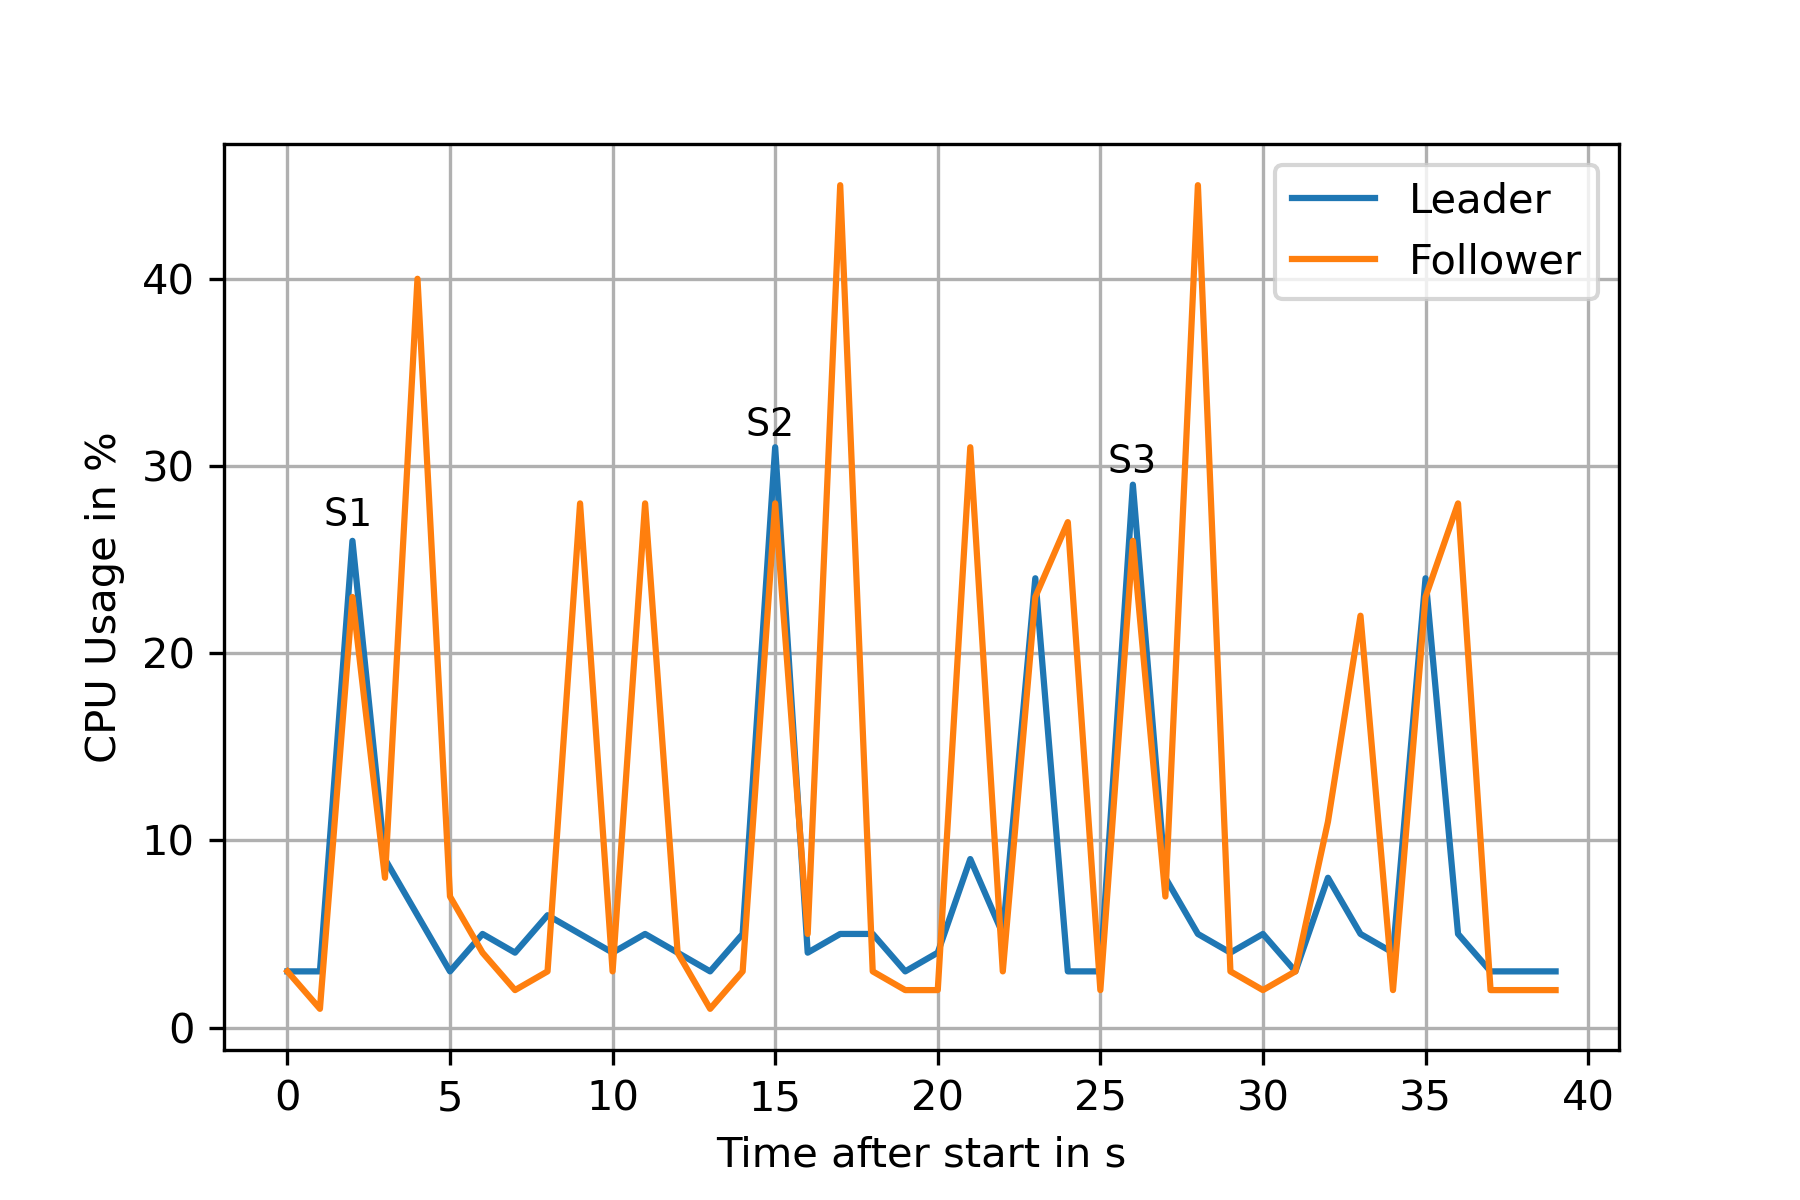
\includegraphics[width=0.75\linewidth]{images/plots/CPUUsage}
	\caption{This plot shows the \glsentryfull{CPU} utilization in \% for both leader and follower while the system receives and evaluates input messages.}
	\label{fig:PlotCPUUsage}
\end{figure}

The \abr{CPU} utilization in operative mode is depicted in~\autoref{fig:PlotCPUUsage}.
For this measurement, three scenarios, namely \textit{Reach End of \abr{MA}}, \textit{Unlinked Balise}, and \textit{Balise not where expected} where run and the resource utilization has been measured with \texttt{pidstat}.
On average, the leader utilizes 7.4\% of the applied \abr{CPU} resources, while a follower utilizes 12.675\% on average.
In system mode, 1.65\% are used for the leader and 1.05\% for a follower on average.
For user mode, the leader utilizes on average 5.73\%, while a follower uses 11.63\%.
\todo{Explain why follower might have higher CPU utilization}

The simulation starts with the first scenario, namely \texttt{Reach End of \abr{MA}}.
The leader's first peak after two seconds (S1) is due to the balise and linking information of the first scenario being evaluated.
At the same time, the followers compare the train's braking curve with the new \abr{MA}, for which the \texttt{MovementAuthority} topic is accessed and the first peak on the follower side can be explained.
After four seconds, the follower has another peak in \abr{CPU} utilization.
At this point, the first balise is encountered and the train's position is compared to the linked balises.
Therefore, the train's state and the linked balises are retrieved for the first time from the topic, which together with the decision making leads to a high computational overhead.
The third and fourth peak (after nine and eleven seconds) are again due to an evaluated balise telegram.
However, only the updated train state is retrieved.

The seconds scenario - \texttt{Unlinked Balise} - starts after 15 seconds (\textbf{S2}).
The peaks can again be explained by data publication and retrieval.
At 23 seconds after the measurements started, the unlinked balise is encountered and the train needs to stop.
This leads to an increase in \abr{CPU} utilization for both the leader and the followers.

The third scenario - \texttt{Balise not where expected} - starts at 26 seconds (\textbf{S3}).
At 35 seconds after the measurements were started, the unexpected balise has been encountered, which can be seen in the graph as well.

\subsubsection{Message Exchanges}
\todo{Mention that Hauptlast is on leader (see total received and sended)}
As the scenarios are run, messages are exchanged between the replicas via the different \abr{DDS} topics.
In the following, the exchange of messages that occur during the simulation of the three successive scenarios from~\autoref{tab:simulatedScenarios} is analyzed.
At first, all messages that were sent by a replica are examined.
Therefore, the total number of sent messages, as well as the number of messages for the consensus topics and the state topics are analyzed.
Afterwards, the same is done for all messages that were consumed by a replicy.

After running the scenarios and recording message sending and receiving events for 25 seconds, the system's leader has been manually stopped.
Thus, the third scenario has been run only with a leader and one follower, instead of a leader and two followers for the first two scenarios.
\\

For the message exchange evaluation, the leader has been manually stopped after the second scenario and before the third scenario is run.
The third scenario has been run with only a leader and one follower.
Any active hardware redundancy mechanisms have been disabled to show how the system elects a new leader, continues its operation, and fulfills the desired behaviour with two instead of three replicas.
In a later section, the active hardware redundancy features will be reactivated to show its effects on the system's reliability.
For each measurement, the heartbeat timer has been set to 100000µs so that ten messages per second can be attributed to heartbeat messages.

\paragraph{Total Messages Sent}

\begin{figure}[!hb]
	\centering
	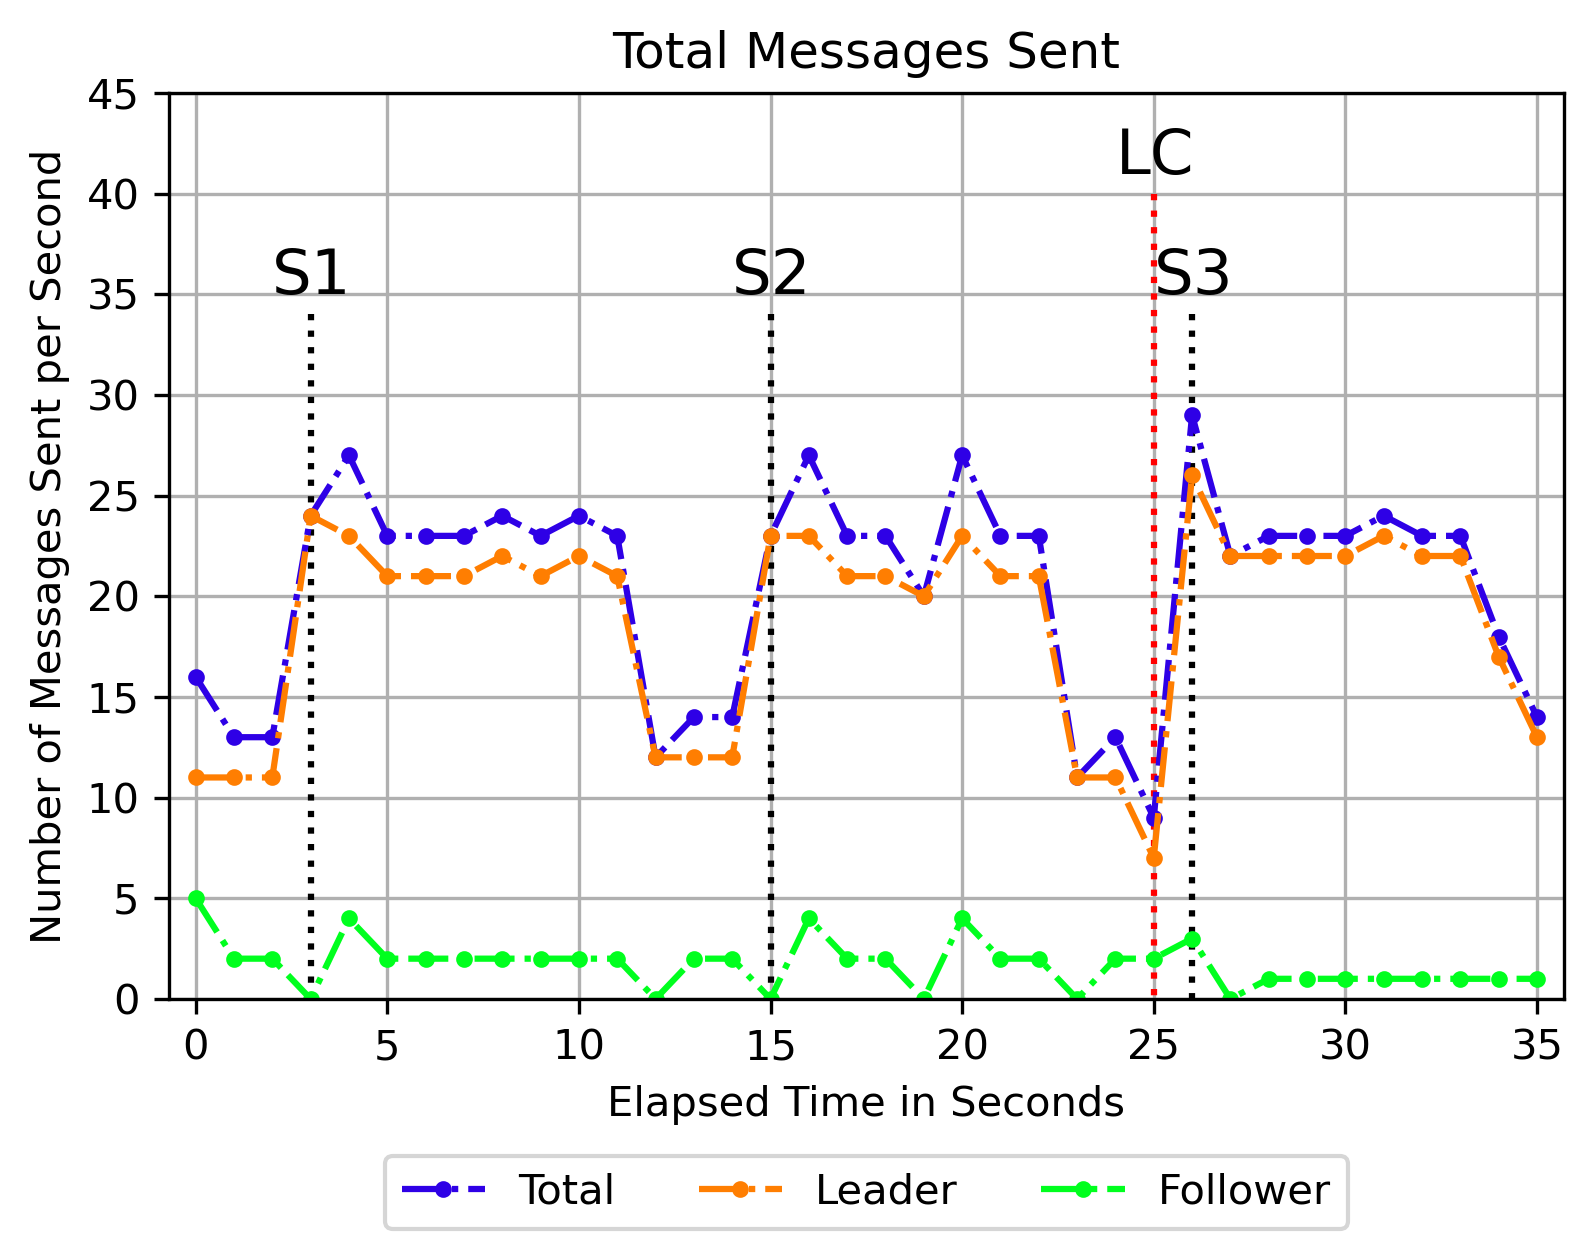
\includegraphics[width=0.75\linewidth]{images/plots/TotalMessagesSent}
	\caption{Overview about all messages that were send in the system. A distinction is made between the messages that were send by the system's leader and the followers. In addition, the overall number of sent messages is shown.}
	\label{fig:PlotTotalMessagesSent}
\end{figure}

The total number of messages that were send by the replicas per seconds is shown in~\autoref{fig:PlotTotalMessagesSent}.
Beginning and end of each of the three scenarios can be seen in the plot by means of the total number of sent messages.
While the train is driving, 20-25 messages were send per seconds.
The number reduces to twelve messages per seconds when the scenarios finish, the train stops, and the system returns to idle mode.
While the train is driving, it is the leader's responsibility to update the system's global state which explains the big increase in sent messages during operation.
A majority of messages is sent by the system's leader of which ten alone are due to heartbeat messages.
The rest accrue from a system-wide braking curve monitoring, for which decicisions were transmitted.

\paragraph{Operative Messages Sent}

VON HIER AUS WEITER MACHEN!!

\begin{figure}[!hb]
	\centering
	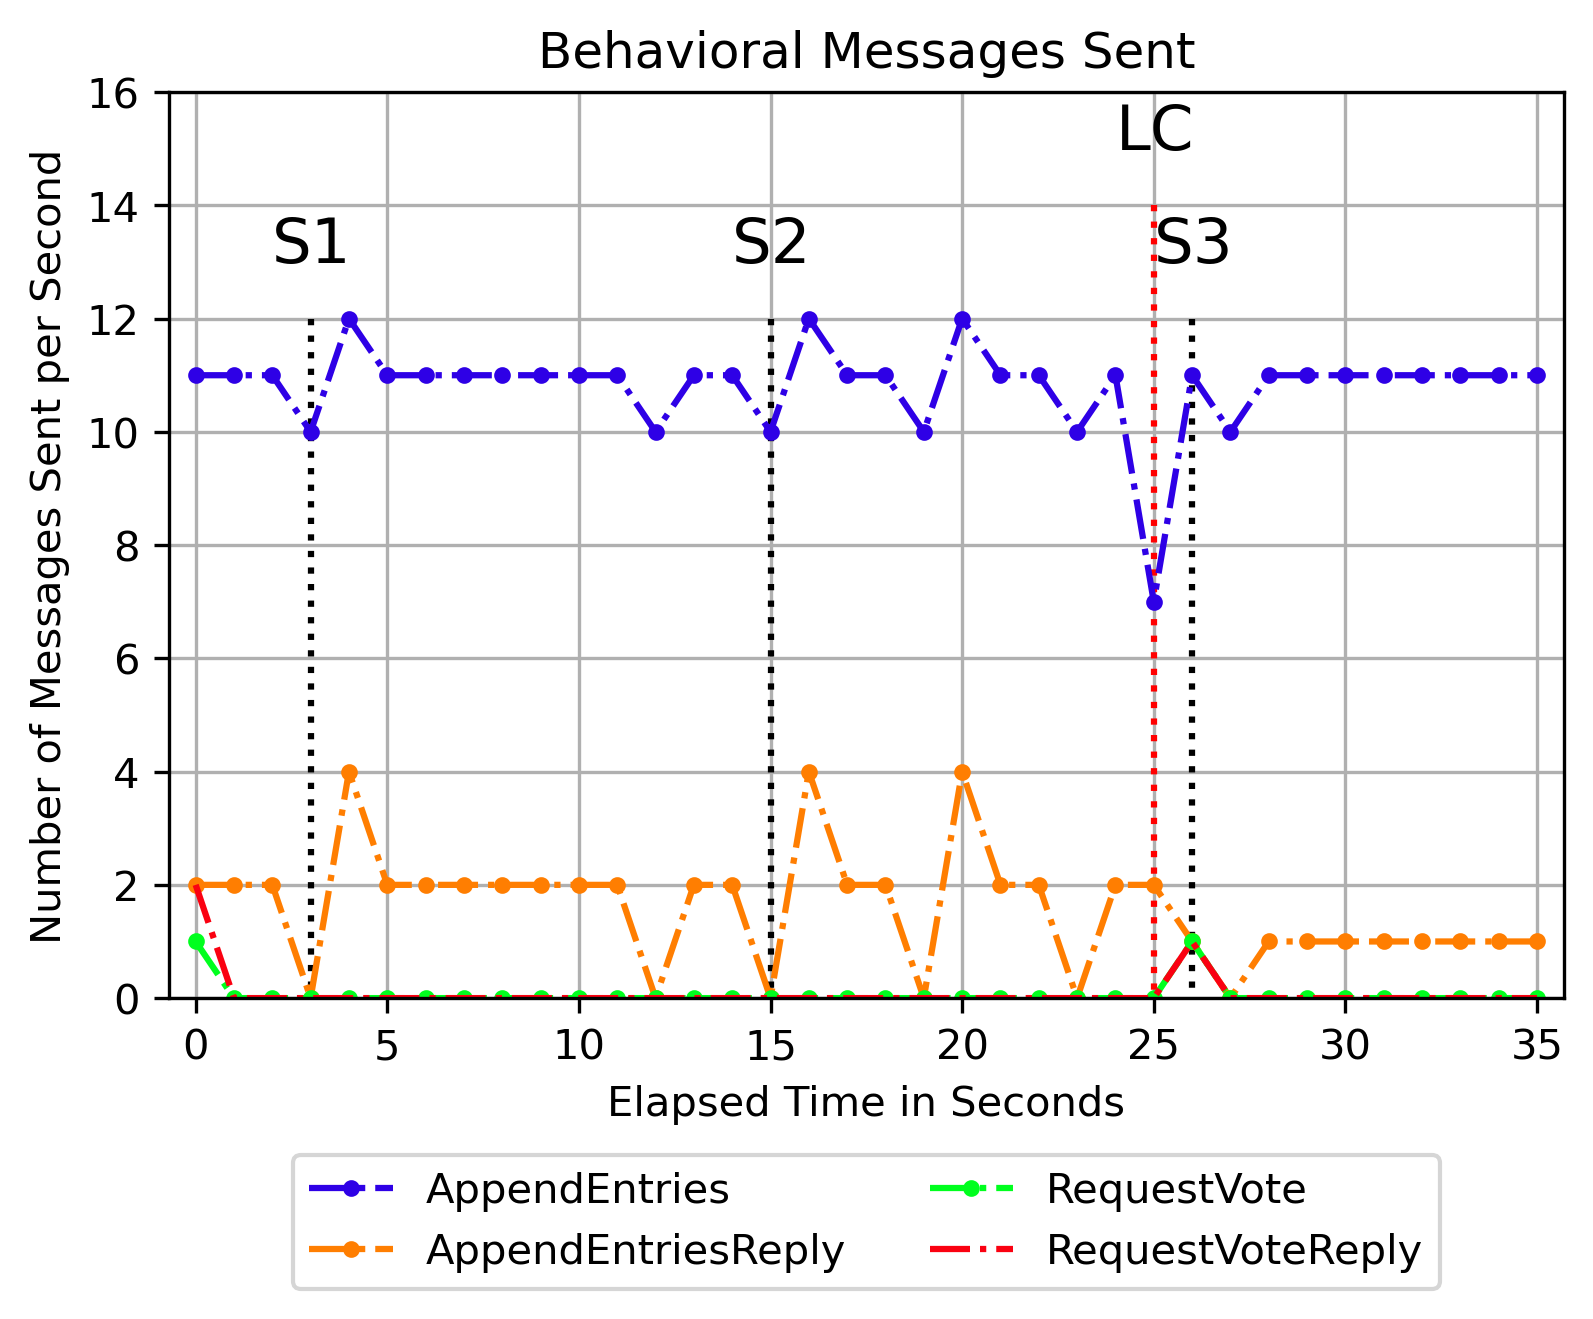
\includegraphics[width=0.75\linewidth]{images/plots/ConsensusMessagesSent}
	\caption{The sent messages for all topics that are used by the consensus and the input processing component. \texttt{AppendEntries} is used for heartbeat messages and for log replication. \texttt{AppendEntriesReply} functions as a way to transmit decisions from followers to the leader. Via \texttt{RequestVote} and \texttt{RequestVoteReply}, the leader election happens. After 25 seconds, the previous leader crashes, which results in a drop of heartbeat messages in the \texttt{AppendEntries} topic. After a new leader is elected, the amount of heartbeat messages goes back to the previous amount.}
	\label{fig:PlotConsensusMessagesSent}
\end{figure}

Operative topics include \texttt{AppendEntries}, \texttt{AppendEntriesReply}, \texttt{RequestVote}, and \texttt{RequestVoteReply}.
The number of messages published to these topics are depicted in~\autoref{fig:PlotConsensusMessagesSent}.
The majority of messages gets published to the \texttt{AppendEntries} topic because the leader periodically published a heartbeat message every 100000µs.
Before the first scenario is executed, a leader election takes place which is indicated by traffic on \texttt{RequestVote} and \texttt{RequestVoteReply}.
Another leader election happens after the second scenario has finished after 25 seconds.
The fact that the previous leader crashed is reflected in the collapse of heartbeat messages on the \texttt{AppendEntries} topic.
Again, a vote request is published to the corresponding topic by the first replica that notices the absent leader.
This time, only one vote reply is published because only one other replica remains in the system.
The fact that the amount of heartbeat messages increases back to the number before the previous leader crashed indicates that a new leader has been established.

\paragraph{State Messages Sent}

\begin{figure}[!hb]
	\centering
	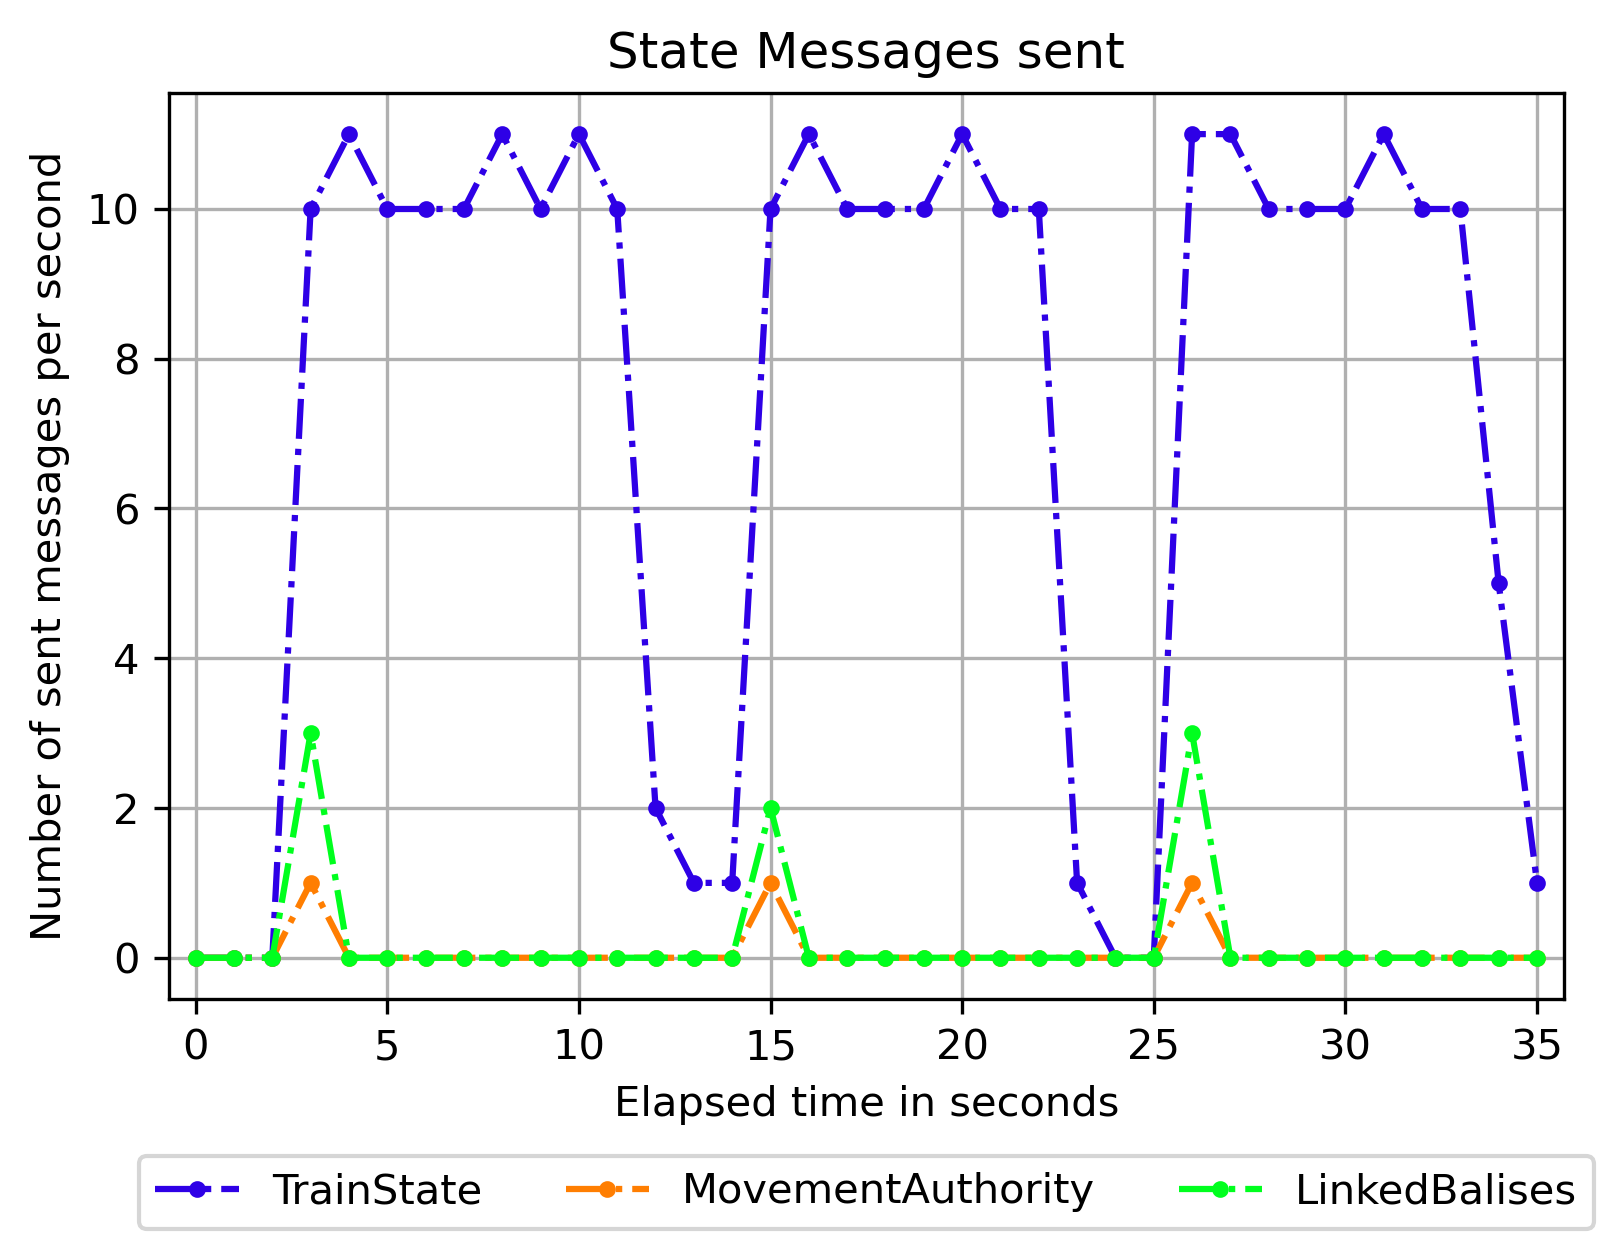
\includegraphics[width=0.75\linewidth]{images/plots/StateMessagesSent}
	\caption{The sent messages for the topics that store the system's global state. It can be seen that, at the beginning of each scenario, a new \glsentryfull{MA} and linked balises are stored. The train's position is simulated and updated every 100ms in the \texttt{TrainState} topic.}
	\label{fig:PlotStateMessagesSent}
\end{figure}

State topics include \texttt{TrainState}, \texttt{MovementAuthority}, and \texttt{LinkedBalises}.
The amount of messages published to these topics can be seen in~\autoref{fig:PlotStateMessagesSent}.
These messages are all sent by the leader, because it is the only replica that is allowed to publish to these topics.
It is noticeable that most state messages are published on the \texttt{TrainState} topic.
This is because the position is simulated every 100000µs and written to \texttt{TrainState}.
The small peaks for the \texttt{TrainState} topic indicate that the train's position is reset when the train encounters a linked balise.
Messages to \texttt{MovementAuthority} and \texttt{LinkedBalises} are only published at the beginning of each scenario, because at this time the \abr{MA} and linked balises are communicated to the system.
It can futher easily be seen that three balises are linked in the first and the third scenario but only two linked balises are added for the second.

\paragraph{Total Messages Received}

\begin{figure}[!hb]
	\centering
	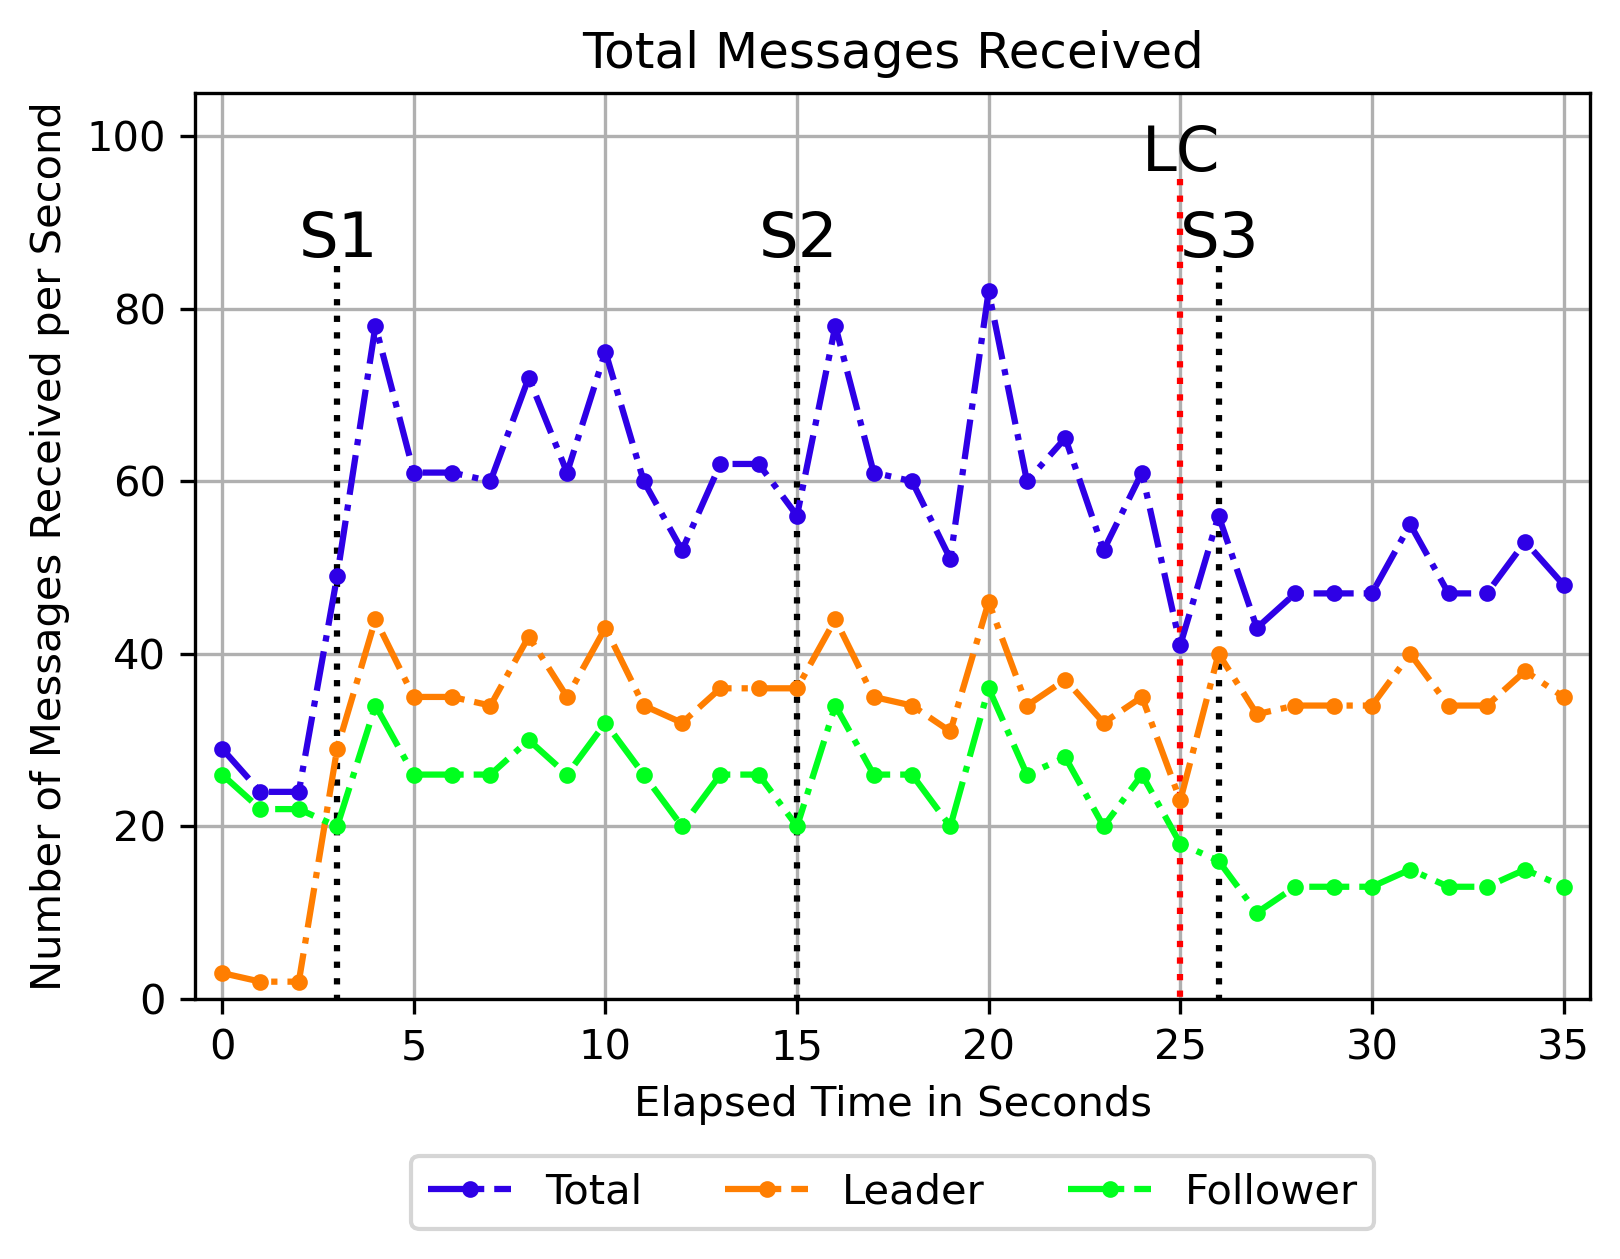
\includegraphics[width=0.75\linewidth]{images/plots/TotalMessagesReceive}
	\caption{Overview about all messages that are received from replicas within the system.}
	\label{fig:PlotTotalMessagesReceive}
\end{figure}

The total number of messages received through \abr{DDS} topics can be seen in~\autoref{fig:PlotTotalMessagesReceive}.
What is interesting is, that the leader receives and reads more messages than the two followers combined.
This is mostly because the leader is responsible for reading the input topic and because it receives and reads messages from both followers.
Another interesting circumstance can be seen after 25 seconds - which is when the previous leader crashes - since the amount of messages that the followers received is halved.
This is because only one, instead of two, followers remain in the system.

\paragraph{Input Messages Received}

\begin{figure}[!hb]
	\centering
	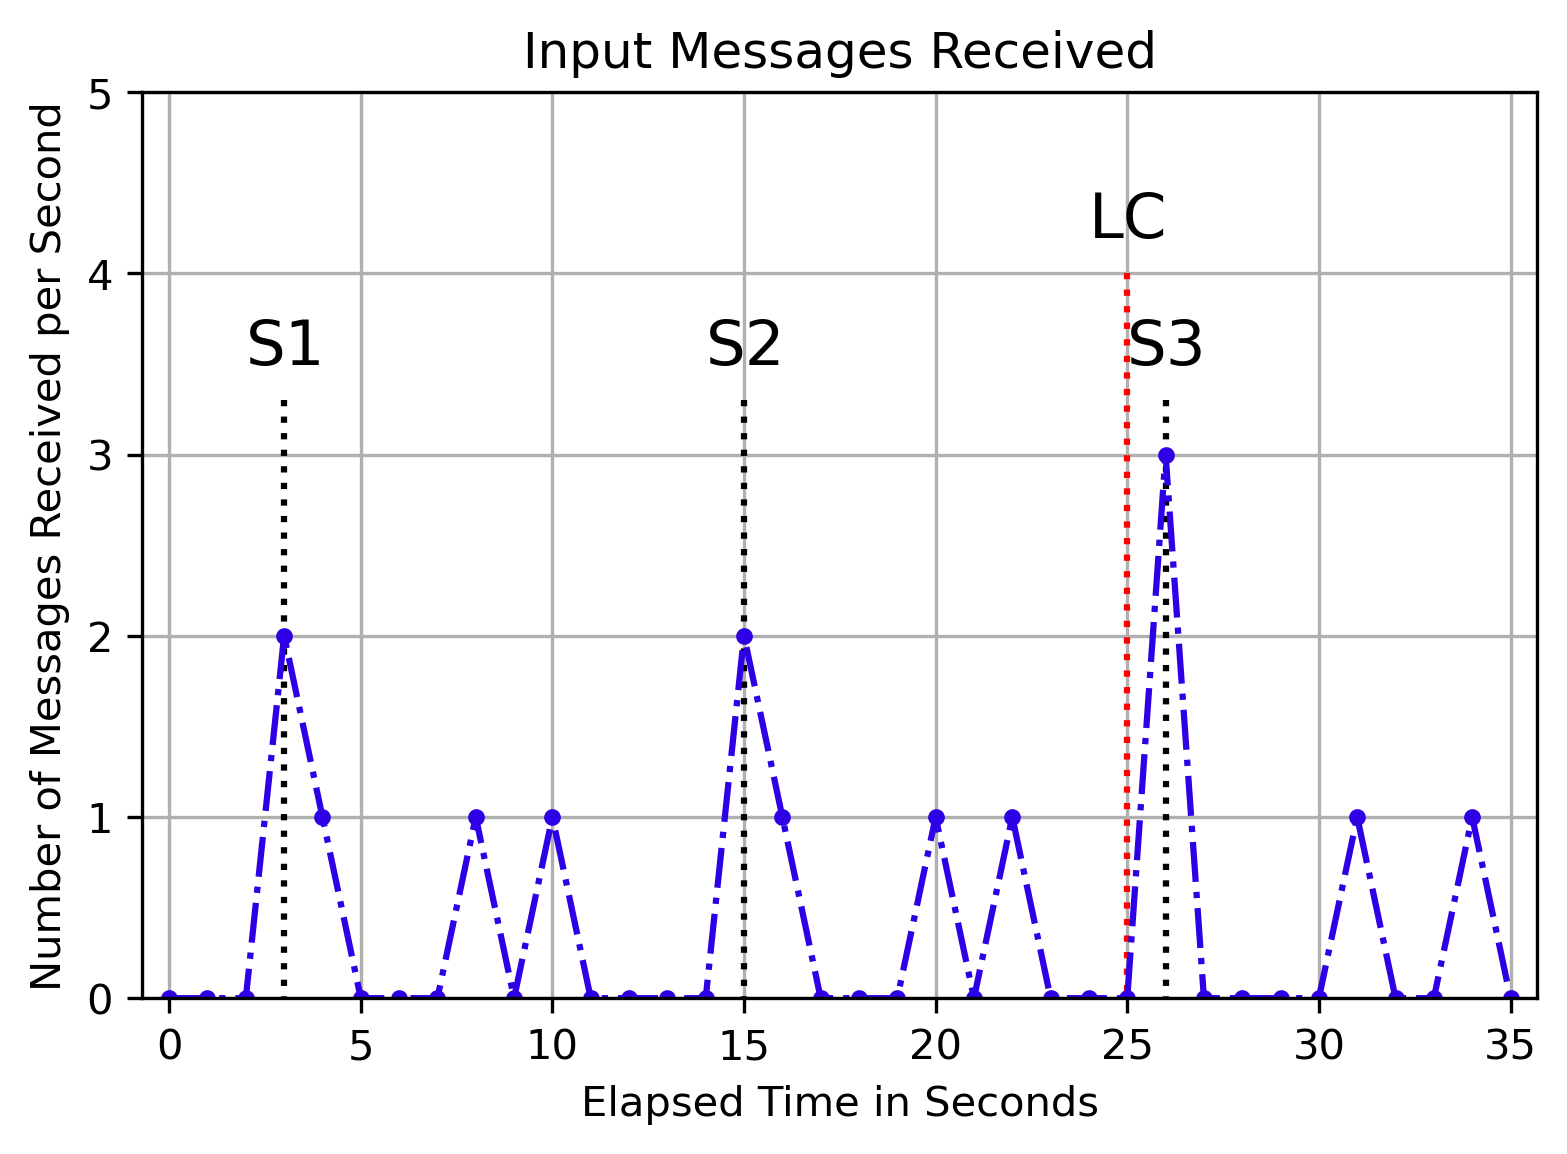
\includegraphics[width=0.75\linewidth]{images/plots/InputMessagesReceive}
	\caption{The number of input messages received by the system per second. Based on the distribution the scenarios procedure can be seen. At the beginning, two input messages contain the \glsentryfull{MA} and linked balises. One second later, the first balise telegram is received. The last two balise telegrams follow each other at an interval of two seconds. The distance between the last two balises is greater for the last scenario. This is because the last scenario, it is simulated that the balise is not at the position that was specified in the linking phase.}
	\label{fig:PlotInputMessagesReceive}
\end{figure}

The individual scenarios' structures can be traced by the input messages that the sytem receives.
This is depicted in~\autoref{fig:PlotInputMessagesReceive}.
At the beginning of each scenario, one message with the \abr{MA} and one with the linked balises are sent.
Because the train's speed is simulated to be constant, the intervals between the incoming balises telegrams are the equal for the first and the second scenario.
In the third scenario it is simulated that the last balise is at a different position than specified in the linking phase.
Therefore, the distance between the last two balises is greater in the third scenario.
It can also be seen that although after 25 seconds the old leader crashes, the system does not miss any input message.
However, unlike the first two scenarios, the input messages are buffered and therefore processed all at once, which is why the peak is higher.

\paragraph{Consensus Messages Received}

\begin{figure}[!hb]
	\centering
	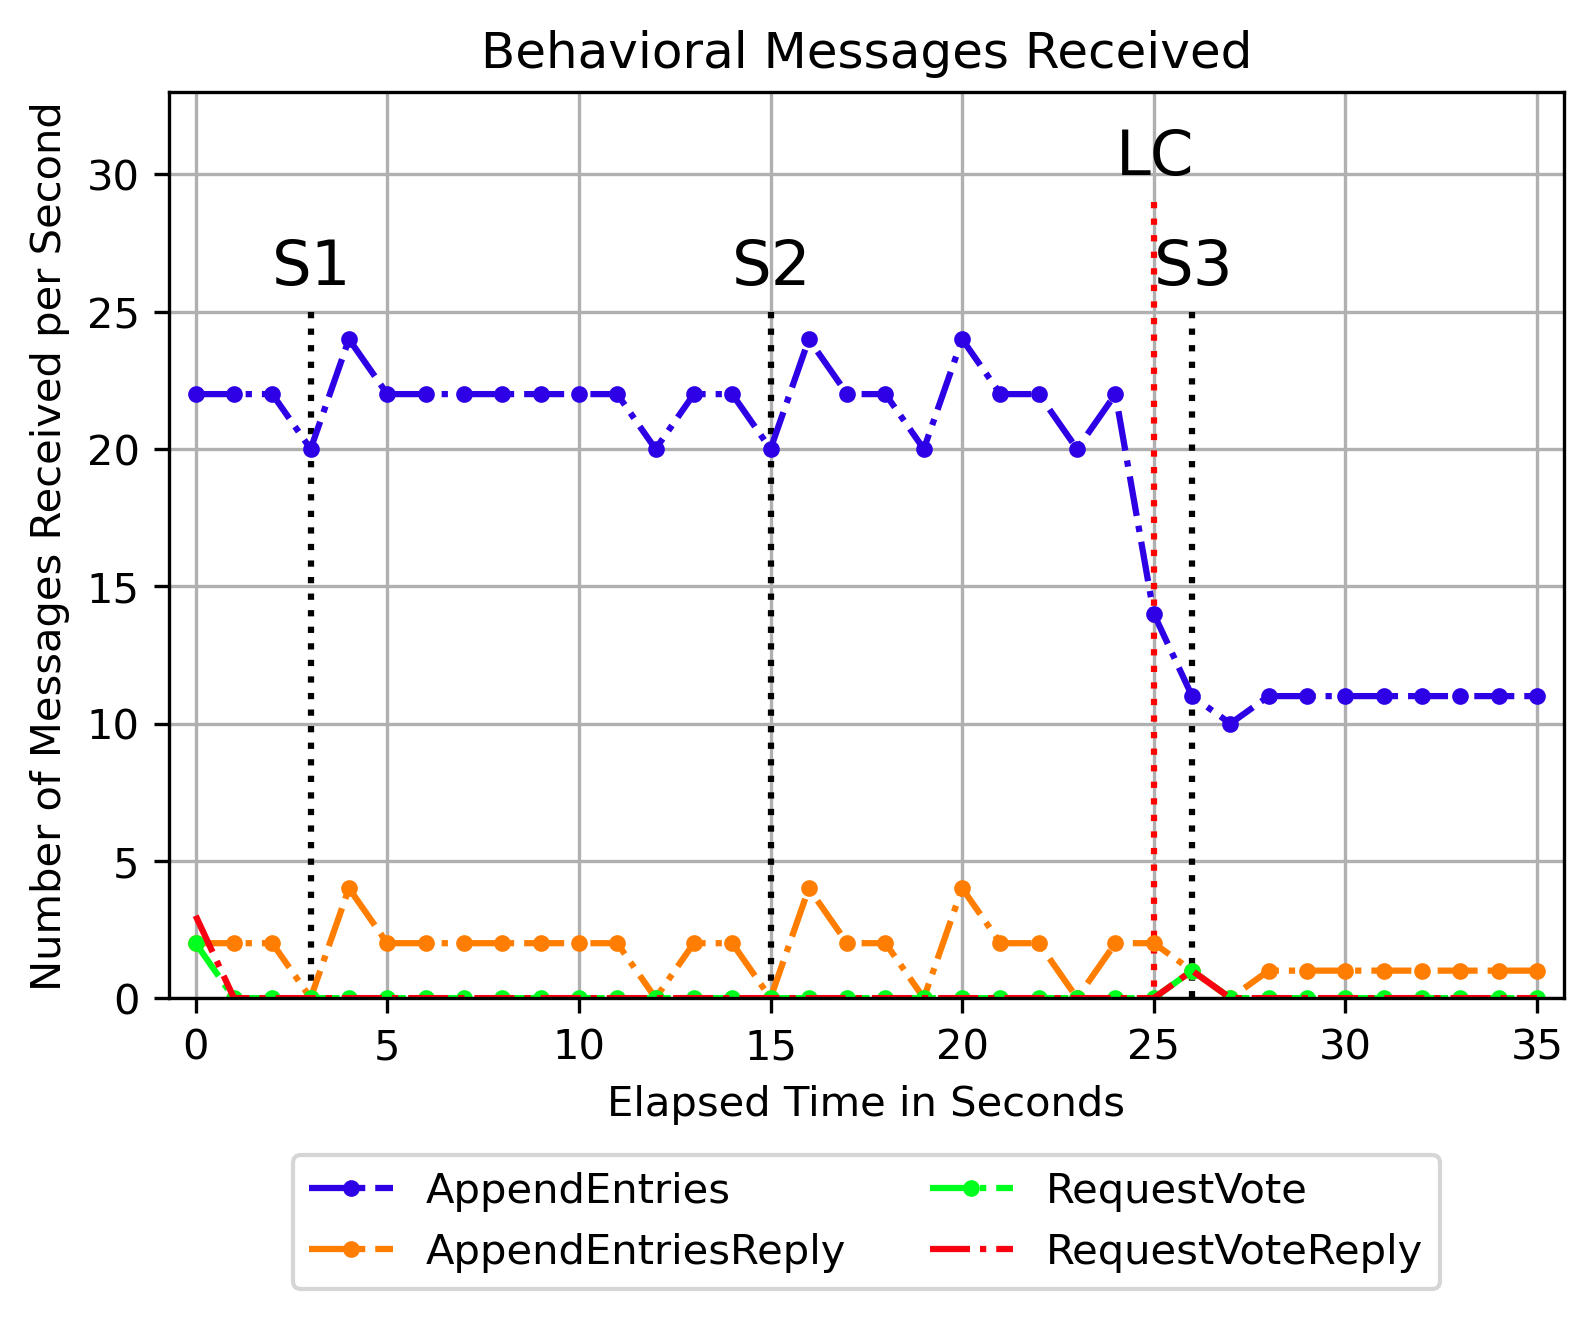
\includegraphics[width=0.75\linewidth]{images/plots/ConsensusMessagesReceive}
	\caption{All messages that are received by a component on the topics used for finding a consensus. After 25 seconds, a new leader is elected and only one follower remains in the system. Therefore, messages are read from \texttt{RequestVote} and \texttt{RequestVoteReply}. Further, since the number of followers got reduced by half, also the number of received heartbeat messages got reduced.}
	\label{fig:PlotConsensusMessagesReceive}
\end{figure}

The number of received messages on the consensus topics is shown in~\autoref{fig:PlotConsensusMessagesReceive}.
It is noticeable that after 25 seconds the number of AppendEntries messages received drops.
Further, a message is received on the \texttt{RequestVote} and on the \texttt{RequestVoteReply} topic, respectively.
From this it can be seen that a leader election occurred.
Because there is only one follower left in the system, the number of received heartbeat messages is halved.

\paragraph{Active Hardware Redundancy}

\begin{figure}[!hb]
	\centering
	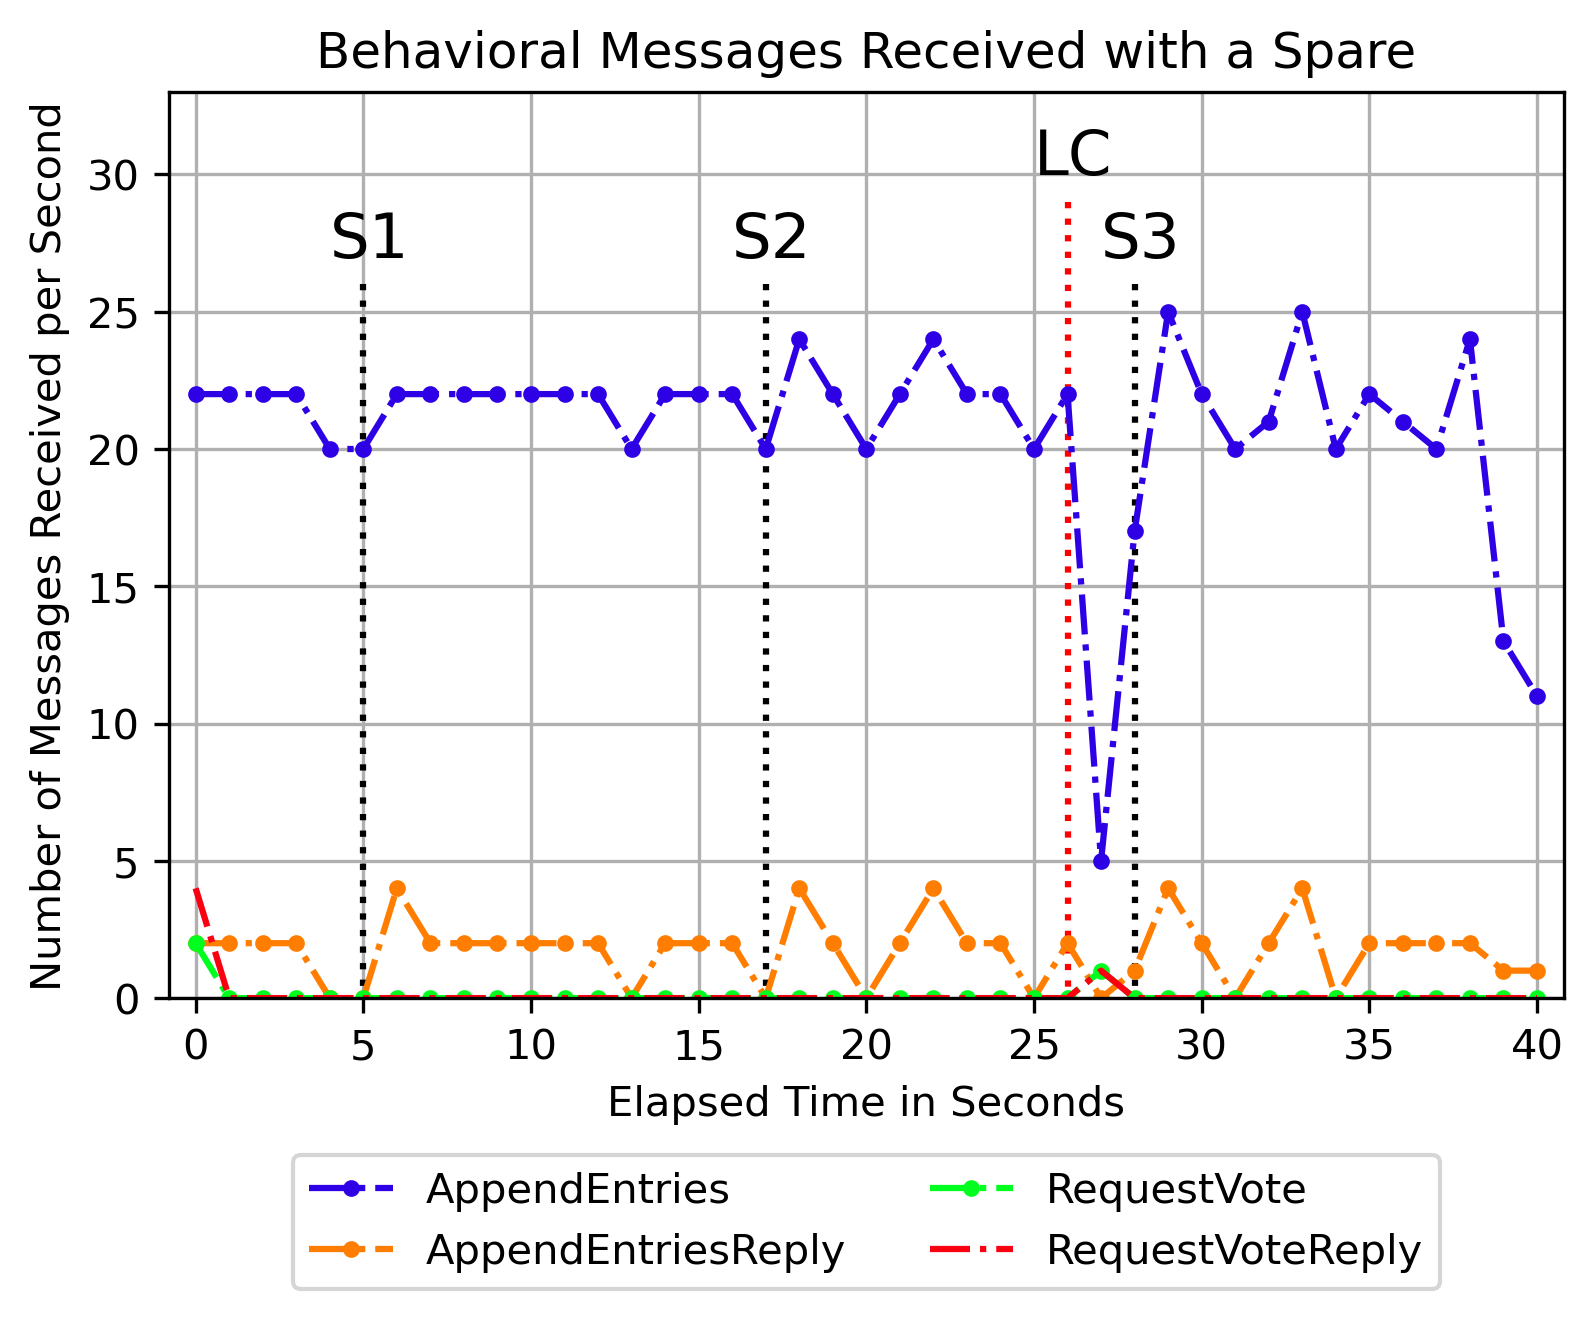
\includegraphics[width=0.75\linewidth]{images/plots/ConsensusMessagesReceiveAHR}
	\caption{All messages that are received by components used by the input processing and consensus module with applied active hardware redundancy. After 27 seconds, the previous leader crashed, a new one is elected and the spare is activated. Hence, the number of received heartbeat messages dropps and goes back the the previous value afterwards.}
	\label{fig:PlotConsensusMessagesReceiveAHR}
\end{figure}

The total number of messages that are received via the consensus topics is depicted in~\autoref{fig:PlotConsensusMessagesReceiveAHR}.
As for the experiment depicted in~\autoref{fig:PlotConsensusMessagesReceive}, the leader was terminated manually after editing the second scenario.
This is evident from the collapse of the received heartbeat messages in the system.
Shortly after, a new leader election takes place and the number of received messages on the \texttt{AppendEntries} topic stabilizes.
Unlike in~\autoref{fig:PlotConsensusMessagesReceive}, the number goes back to the original received messages showing that there are three active replicas again.


\subsection{Safety and Reliability}
The redundant and distributed system has been designed to be reliable and safe.
Reliability has been defined as a probability that a system functions as specified over a period of time (see~\autoref{def:reliability}).
It has been increased using \abr{TMR}, which enhances a system's fault-tolerance though error masking, and with active hardware redundancy to replace faulty components.
Thereby, transient and permanent hardware faults, the main source of hardware malfunctions, are covered~\cite{MULAZZANIReliabilityVsSafety}.

However, software fails due to design faults.
The software system's reliability has been shown through acceptance tests via simulation and replication of reproducable test scenarios.

In contrast to reliability, safety aims at the avoidance of catastropic failures (\autoref{def:safety}).
Throughout this thesis, all safety considerations have been made with the assumption of a functioning and safe communication layer.
The system's safety has been enhanced by applying a hybrid of consensus and voting based approaches to prevent the voter from being a single point of failure.
Further, the presence of a leader is guaranteed because the system counts the number of failed leader election cycles and every leader permanently listens for heartbeat messages from other leaders.
Thereby, the train can be stopped when the system is without a leader for too long and a split brain situation can be detected.
The situation of a system wide power outage can be diminished by using a distingt power source for each replica.
If a power failure does occur, physical components such as gravity switches could be used to prevent the system's environment to be harmed.

A balise in the wrong place or an unlinked balise can also be a safety hazard.
These threats are be addressed by the system's functional logic and are proven to be prevented in the acceptance tests, even in case of individual component failures.

\section{\glsentrylong{DDS} Evaluation}
\todo{Summarize how the subset looks like}
\abr{DCPS} systems, such as \abr{DDS}, are designed for machine-to-machine communication in real-time applications~\cite{omgDDSspec}.
It builds upon a decoupling from senders and receivers to facilitate a flexible and scalable system.
However, decoupling of senders and receivers is not always possible in a consensus-based and safety-critical redundant system because a follower replica that receives heartbeat messages can become sender of heartbeat messages at any time when the previous leader becomes unavailable.

Further, \abr{DDS} is designed as a standard for distributed application communication and integration and therefore implements variety of features.
Not all of these features are required for a system like the one that is assessed in this work.
\\

Therefore in this section, a feature subset of ADLINK's \texttt{OpenSplice DDS} is presented that is sufficient to implement the requirements placed on the system.
Afterwards, the suitability of \abr{DDS} for safety-critical and consensus-based redundant systems is discussed.
\subsection{\glsentrylong{DDS} Subset Identification}

For reducing costs incurred in the system approving process, it is important to limit the amount of utilized features and lines of code.
Therefore, a subset of \abr{DDS} features from OpenSplice DDS, that is sufficient for building a redundant system, is identified.
An overview about this subset is given and justified in the following.
This overview only contains the methods and functionalities that are directly used by the application, the middleware, however, might utilize other functionalities to implement the features mentioned in this section.

\paragraph{Domain Module}
A \abr{DDS} application's main building blocks comprise a \texttt{Domain}, one or multiple \texttt{DomainParticipants}, as well as a \texttt{DomainParticipantFactory} for creating new \texttt{DomainParticipants}~\cite{omgDDSspec}.
Besides these classes, the domain module contains various functionalities, from which only the following subset is used within the exemplary implementation.

\begin{itemize}
\item \textit{DDS\_Entity\_get\_instance\_handle} Is used for acquiring an instance handle to mark it as processed in the leader's commit phase.
\item \textit{DDS\_DomainParticipant\_create\_(publisher|subscriber|topic)} Is used for creating \abr{DDS} publishers, subscribers or topics.
\item \textit{DDS\_DomainParticipant\_delete\_(publisher|subscriber|topic)} Is used for deleting \abr{DDS} publishers, subscribers or topics.
\item \textit{DDS\_DomainParticipantFactory\_get\_instance} Used for acquiring the \texttt{DomainParticipantFactory} singleton.
\item \textit{DDS\_DomainParticipantFactory\_(create|delete)\_participant} Used for creating a new participant in the \abr{DDS} domain.
\end{itemize}

Even though \textit{DDS\_DomainParticipant\_get\_default\_(publisher|subscriber|topic)\_qos} is used in the implementation, it is not mandatory because one could set the default \abr{QOS} settings directly on the corresponding entity.

\paragraph{Topic-Definition Module}
The topic definition module contains everything related to topics.
The exemplary implementation utilizes \texttt{Topics}, for describing data in the application, and \texttt{TypeSupport} which describes a data type that is bound to a \texttt{Topic}.
Apart from these two classes, the following methods are used:

\begin{itemize}
\item \textit{DDS\_TypeSupport\_\_alloc} Used for creating a new \texttt{TypeSupport}.
\item \textit{DDS\_TypeSupport\_get\_type\_name} Used for getting a data type's default name, which is required to register it later on.
\item \textit{DDS\_TypeSupport\_register\_type} Used for registering a new data type name on a \texttt{DomainParticipant}.
\end{itemize}


\paragraph{Publication Module}
\texttt{Publishers}, as well as \texttt{DataWriters}, which are used for data distribution, are located within the publication module.
Besides these two classes, the following functionality is required for the exemplary implementation:

\begin{itemize}
\item \textit{DDS\_Publisher\_(create|delete)\_datawriter} Used for creating, respectively deleting, \texttt{DataWriter} objects.
\item \textit{DDS\_DataWriter\_write} Used for writing new data to an instance on a \abr{DDS} topic.
\item \textit{DDS\_DataWriter\_dispose} Used for marking processed inputs for deletion so that they are not processed twice.
\end{itemize}

\textit{DDS\_Publisher\_copy\_from\_topic\_qos} and \textit{DDS\_Publisher\_get\_default\_datawriter\_qos} are not necessarily required due to the same reasons stated above.

\paragraph{Subscription Module}
The subscription module resembles the publication module, but for reading and receiving data.
However, besides \texttt{Subscribers} and \texttt{DataReaders}, it also contains \texttt{DataSample}, \texttt{SampleInfo}, \texttt{ReadCondition}, and \texttt{QueryCondition}, which are utilized in the exemplary implementation.
\texttt{Subscribers} and \texttt{DataReaders} are required for receiving data, which is represented by a \texttt{DataSample}.
The \texttt{SampleInfo} data structure contains additional information for each \texttt{DataSample}, such as its instance handle or state, which makes it mandatory for the implementation as well.
\texttt{ReadConditions} are used in combination with \texttt{WaitSets}, so that the application can react to certain middleware states.
\texttt{QueryConditions} are extensions for \texttt{ReadConditions} that allow to filter the data samples that are covered by a \texttt{ReadCondition}.
All filter operations could be implemented directly in the application code, which would make \texttt{QueryConditions} redundant.

Further, the following functionalities from the subscription module were used:

\begin{itemize}
\item \textit{DDS\_Subscriber\_(create|delete)\_datareader} Used for creating, respectively deleting, \texttt{DataReaders}.
\item \textit{DDS\_DataReader\_(create|delete)\_readcondition} Used for creating, respectively deleting, \texttt{ReadConditions}.
\item \textit{DDS\_DataReader\_create\_querycondition} Used for creating \texttt{QueryConditions}.
\item \textit{DDS\_DataReader\_take\_w\_condition} Used for reading and removing data from a \texttt{DataReader}, filtered by a \texttt{ReadCondition}.
\item \textit{DDS\_DataReader\_return\_loan} Required for indicating the middleware that the application finished accessing a sequence of data. This allows the middleware to work with the data again.
\end{itemize}

\paragraph{Infrastructure Module}
The classes that are used from the infrastructure module include \texttt{QosPolicy} and \texttt{WaitSet}.
The \texttt{QosPolicy} class implements \abr{DDS}'s \abr{QOS} functionalities and is therefore mandatory for the system's correctness.
\texttt{WaitSets} are applied for ensuring the application's compliance with its time restrictions, because they allow the assignment of timeouts.
In addition to that, the following functionalities from the infrastructure module are applied:

\begin{itemize}
\item \textit{DDS\_WaitSet\_\_alloc} Used for creating new \texttt{WaitSets}.
\item \textit{DDS\_WaitSet\_attach\_condition} Used to attach a condition to the corresponding \texttt{WaitSet}.
\item \textit{DDS\_WaitSet\_detach\_condition} Used to detach a condition from the corresponding \texttt{WaitSet}.
\item \textit{DDS\_WaitSet\_wait} Stops the according thread until at least one of the attached conditions evaluates to true.
\end{itemize}

Further, the following \abr{QOS} are applied in the application:
\todo{Add after deciding}

\subsection{Challenges of \glsentrylong{DDS} in Consensus-based Redundant Systems}
In this section, the suitability of \abr{DCPS} systems, like \abr{DDS}, for consensus based redundant systems is discussed.

\paragraph{Advantages}
On the one hand, \abr{DDS} allows to utilize \abr{QOS} settings to specify what is expected from the system rather than how it should be done.
Through \texttt{ReadConditions} and \texttt{QueryConditions}, messages can be filtered.
Further, \texttt{WaitSets} and \abr{QOS}-settings can be used to declare time restriction and requirements.
This facilitates a reliable and predictable machine-to-machine communication.

In addition, the middleware supports automatic discovery of replicas to that the number of used replicas is dynamically scalable.
For example, an active spare unit can be added to the system at any time and is automatically discovered and included.
This would also allow to apply a three-out-of-five system rather than a two-out-of-three system and use the same software.

Finally, \abr{DDS} supports fast transmission times and a manageable hardware utilization, as shown in measurements.

\paragraph{Challenges}
On the other hand, the \abr{DDS} standard has been designed around a loose coupling of publishing and subscribing components.
This is not possible in dynamic systems like the system build in this work.
Because the applied \abr{TMR} builds upon \texttt{Raft}'s leader and log replication concepts, any replica needs to be prepared to become leader or follower at any time.
For example, the system's leader is responsible for publishing heartbeat messages to the \texttt{AppendEntries} topic, while a follower needs to subscribe and receive these heartbeats.
Therefore, replicas are required to dynamically alternate between sending and receiving data.
One way to solve this challenge is to create and delete objects for publishing and subscribing to topics dynamically.
However, this can lead to a sudden allocation and deallocation of dynamic memory which can lead to unpredictable time performances.
Thus, every replica allocates the objects that are required to publish and subscribe to every topic at program start, which leads to other challenges.

When each replica is subscribed to a topic that applies a \texttt{History}- and \texttt{ResourceLimit} \abr{QOS}, the messages that are received by \texttt{DataReader} objects must be taken by the application.
Hence, a leader that is subscribed to the \texttt{AppendEntries} topic in preparation of becoming a follower must take all heartbeat messages from the topic that were published by itself.
This introduces a computational overhead, though a small one as the system's resource utilization in~\autoref{fig:PlotCPUUsageIdleTime} show.

Lastly, a system that utilizes \abr{DDS} for communication needs to support concurrent computations when more that one message should be processable at any time.
This introduces potential race conditions or deadlocks and can complicate the development and approval process.
Since the developed system, for example, needs to react to vote requests and log replication messages at any time, a concurrent system design is unavoidable.
As discussed in~\autoref{subsub:raceConditions} though, the implemented system applies a race condition free concurrent algorithm.

\iffalse
\paragraph{State Messages Received}

\begin{figure}[!hb]
	\centering
	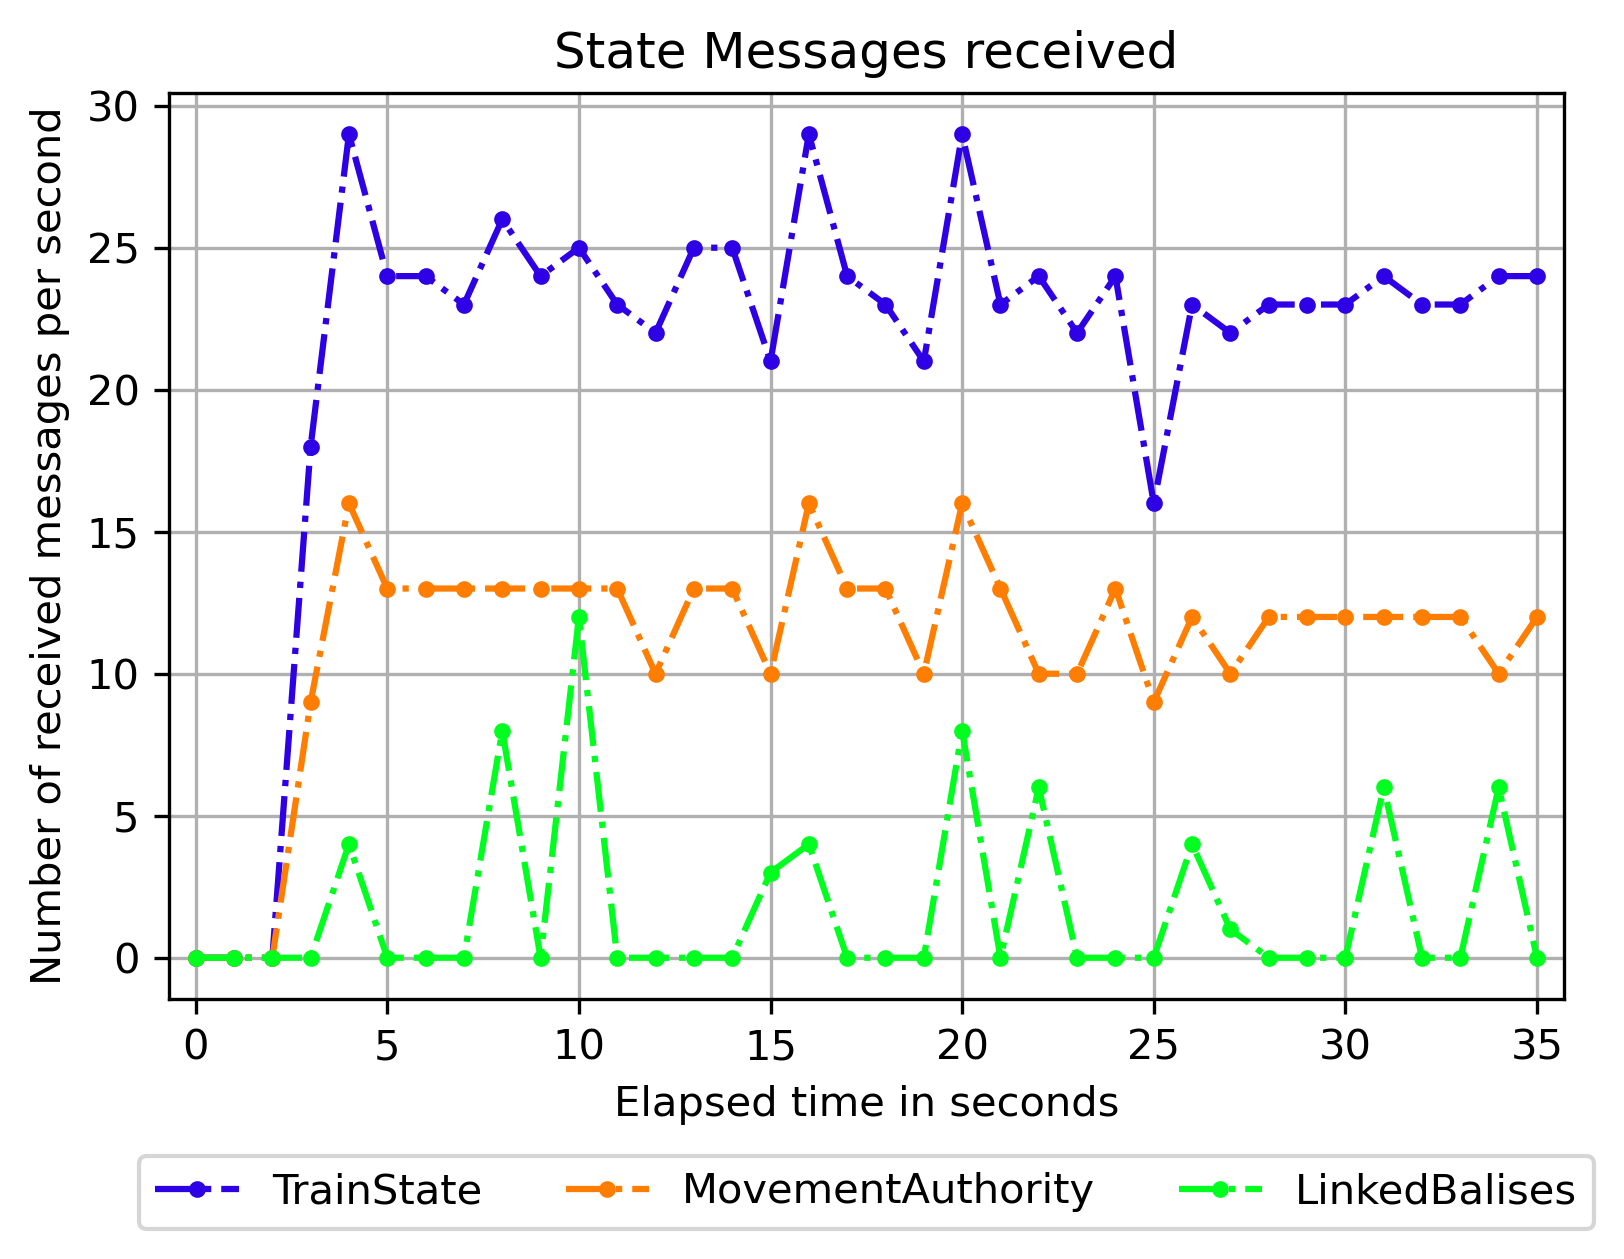
\includegraphics[width=0.75\linewidth]{images/plots/StateMessagesReceive}
	\caption{}
	\label{fig:PlotStateMessagesReceive}
\end{figure}

\todo{Do measurement with killing leader, but this time activate spare and show a topic selection that hot standby works}

Do experiement and structure in way such as SakicTimeInConsensus

Leader stable for 45 minutes with 500000x07x2

For the tranmit time, I measured 20 messages each time and took the average (calculate standard deviation)
\fi
